
\subsection{\textbf{Hadronic physics}}\label{sec:hadphys}
\Gfour{} hadronic physics is loosely defined to cover any reaction which can
produce hadrons in its final state.  As such, it covers purely hadronic
interactions, lepton- and gamma-induced nuclear reactions, and radioactive
decay.  The interaction is represented as a \Gfour{} process which consists of
a cross section to determine when the interaction will occur, and a model which
determines the final state of the interaction.    

Models and cross sections are provided which span an energy range from sub-eV to
~TeV.  Following the toolkit philosophy, more than one model or process is 
usually offered in any given energy range in order to provide alternative 
approaches for different applications. 

During the last several years, new models and cross sections have been added
to the toolkit, while others have been improved and some obsolete models have
been removed.

% shortcut commands for some model names
\newcommand{\incl}{INCL}
\newcommand{\inclxx}{INCL++}
\newcommand{\abla}{ABLA~V3}

%------------------------ Uzhi part ----------------------------------
% A simulation of a particle propagation in a matter requires the following steps:
% a choice of an interaction point and a target nucleus which depend on cross sections
% of the particle interactions with components of the matter, a sampling of a reaction
% of the particle with chosen target nucleus and a simulation of the reaction.
%---------------- Uzhi changes -----------------------------------

\subsubsection{Hadronic cross sections}\label{sec:crosssections}
Total, inelastic and elastic cross sections for hadron-nucleus, nucleus-nucleus
and antinucleus-nucleus reactions are provided which cover energies up to ~TeV 
in some cases.  Proton-, neutron- and pion-nucleus cross sections at low to 
medium energies have been available in \Gfour{} since its beginning and their 
details are covered elsewhere \cite{bib:generalpaper2}.  The focus here is on 
recent developments in cross sections for other projectile types and at higher
energies. \\

% done
%%%%%%%%%%%%%%%%%%%%%%%%%%%%%%%%%%%%%%%%%%%%%%%%%%%
% barashenkov.tex
% Author: Vladimir Grichine
%%%%%%%%%%%%%%%%%%%%%%%%%%%%%%%%%%%%%%%%%%%%%%%%%%%
% \noindent {\emph{Barashenkov cross sections}}
\paragraph{Barashenkov cross sections}
The Barashenkov data set describes proton, neutron and charged pion cross 
sections (total and inelastic) on nuclei~\cite{hadbib:bar90,hadbib:bar89}. 
The Barashenkov interpolation for the total and inelastic cross sections is
essentially based on a quasi-optical model for high energies (T$\,\,>\,\,$2 GeV)
and on phenomenology, with correction terms of the form $\pi r_o A^{2/3}$, 
with $r_o\sim\,\,$1 fm.  The total, inelastic (and elastic) cross sections were
modeled with:
\[
\sigma(T,A)=\pi \left[r_{o}A^{1/3}+\lambda(T,A)\right]^{2}f(T)\phi(A)^{\alpha(T)},
\]
where $\lambda$ is the de Broglie length of the projectile in the center of 
mass system, $T$ is the kinetic energy of the projectile in the lab, $A$ is the 
atomic weight and $r_{o}\sim 1\,\,$fm. 
The functions $f(T)$, $\phi(A)$ and $\alpha(T)$ are series of the form:
\[
\sum_i a_i T^{b_i}\quad\textrm{or}\quad \sum_i a_i A^{b_i}.
\]
The general behavior of the optical models is to predict constant cross sections
for very high energies.  However, experimental data show a moderate relativistic 
rise of hadron-nucleus cross sections.  For this reason the Glauber model was
used to describe hadron-nucleus cross sections in the high energy region (above
90 GeV).


% done
%%%%%%%%%%%%%%%%%%%%%%%%%%%%%%%%%%%%%%%%%%%%%%%%%%%
% glaubergribov.tex
% Author: Gunter Folger, Vladimir Grichine
%%%%%%%%%%%%%%%%%%%%%%%%%%%%%%%%%%%%%%%%%%%%%%%%%%%
\paragraph{Glauber-Gribov extension}
The simplified Glauber model cross sections assume Gaussian-distributed,
point-like nucleons and are given by~\cite{hadbib:ggepjc,hadbib:ggnimb}:
\[
\sigma^{hA}_{tot}=2\pi R^2\ln\left[1+\frac{A\sigma^{hN}_{tot}}{2\pi R^2}\right],\quad
\sigma^{hA}_{in} = \pi R^2\ln\left[1+\frac{A\sigma^{hN}_{tot}}{\pi R^2}\right],
\]
\[
\quad \sigma^{hA}_{el}=\sigma^{hA}_{tot}-\sigma^{hA}_{in}.
\]
Here $\sigma^{hA}_{tot}$, $\sigma^{hA}_{in}$, and $\sigma^{hA}_{el}$ are the
total, inelastic and elastic cross sections, respectively. 

The model is reduced to the selection of $\sigma^{hN}_{tot}$ and $R(A)$
values.  The latest edition of PDG \cite{hadbib:PDG} and \Gfour{} parameterizations
were used for $\sigma^{hN}_{tot}$, including the total cross sections of $p$,
$\bar{p}$, $n$, $\pi^{\pm}$, $K^{\pm}$ and $\Sigma^{-}$ on protons and neutrons
% (http://pdg.lbl.gov/2006/reviews/hadronicrpp.pdf).  
For known cross sections on protons and neutrons,
$A\sigma^{hN}_{tot}=N_{p}\sigma^{hp}_{tot}+N_{n}\sigma^{hn}_{tot}$, where $N_{p}$
and $N_{n}$ are the number of protons and neutrons in the nucleus.
The nuclear radius (the RMS radius of the nucleon Gaussian distribution), 
is parametrized as $R(A) = r_{o}A^{\frac{1}{3}}f(A)$, 
$r_{o} \sim 1.1 \ fm$, with $f(A) < 1$ for $A > 21$, and $f(A) > 1$ for the  
case $3 < A < 21$. 
Figures \ref{nCtotinprodGG} and \ref{pCinprodBGG} show the prediction of the
Barashenkov and Glauber-Gribov model for total, inelastic and production cross
sections of neutrons and protons on a carbon target.  The production cross
section is defined to be the difference between the inelastic and charge 
exchange cross sections.  

\begin{figure}
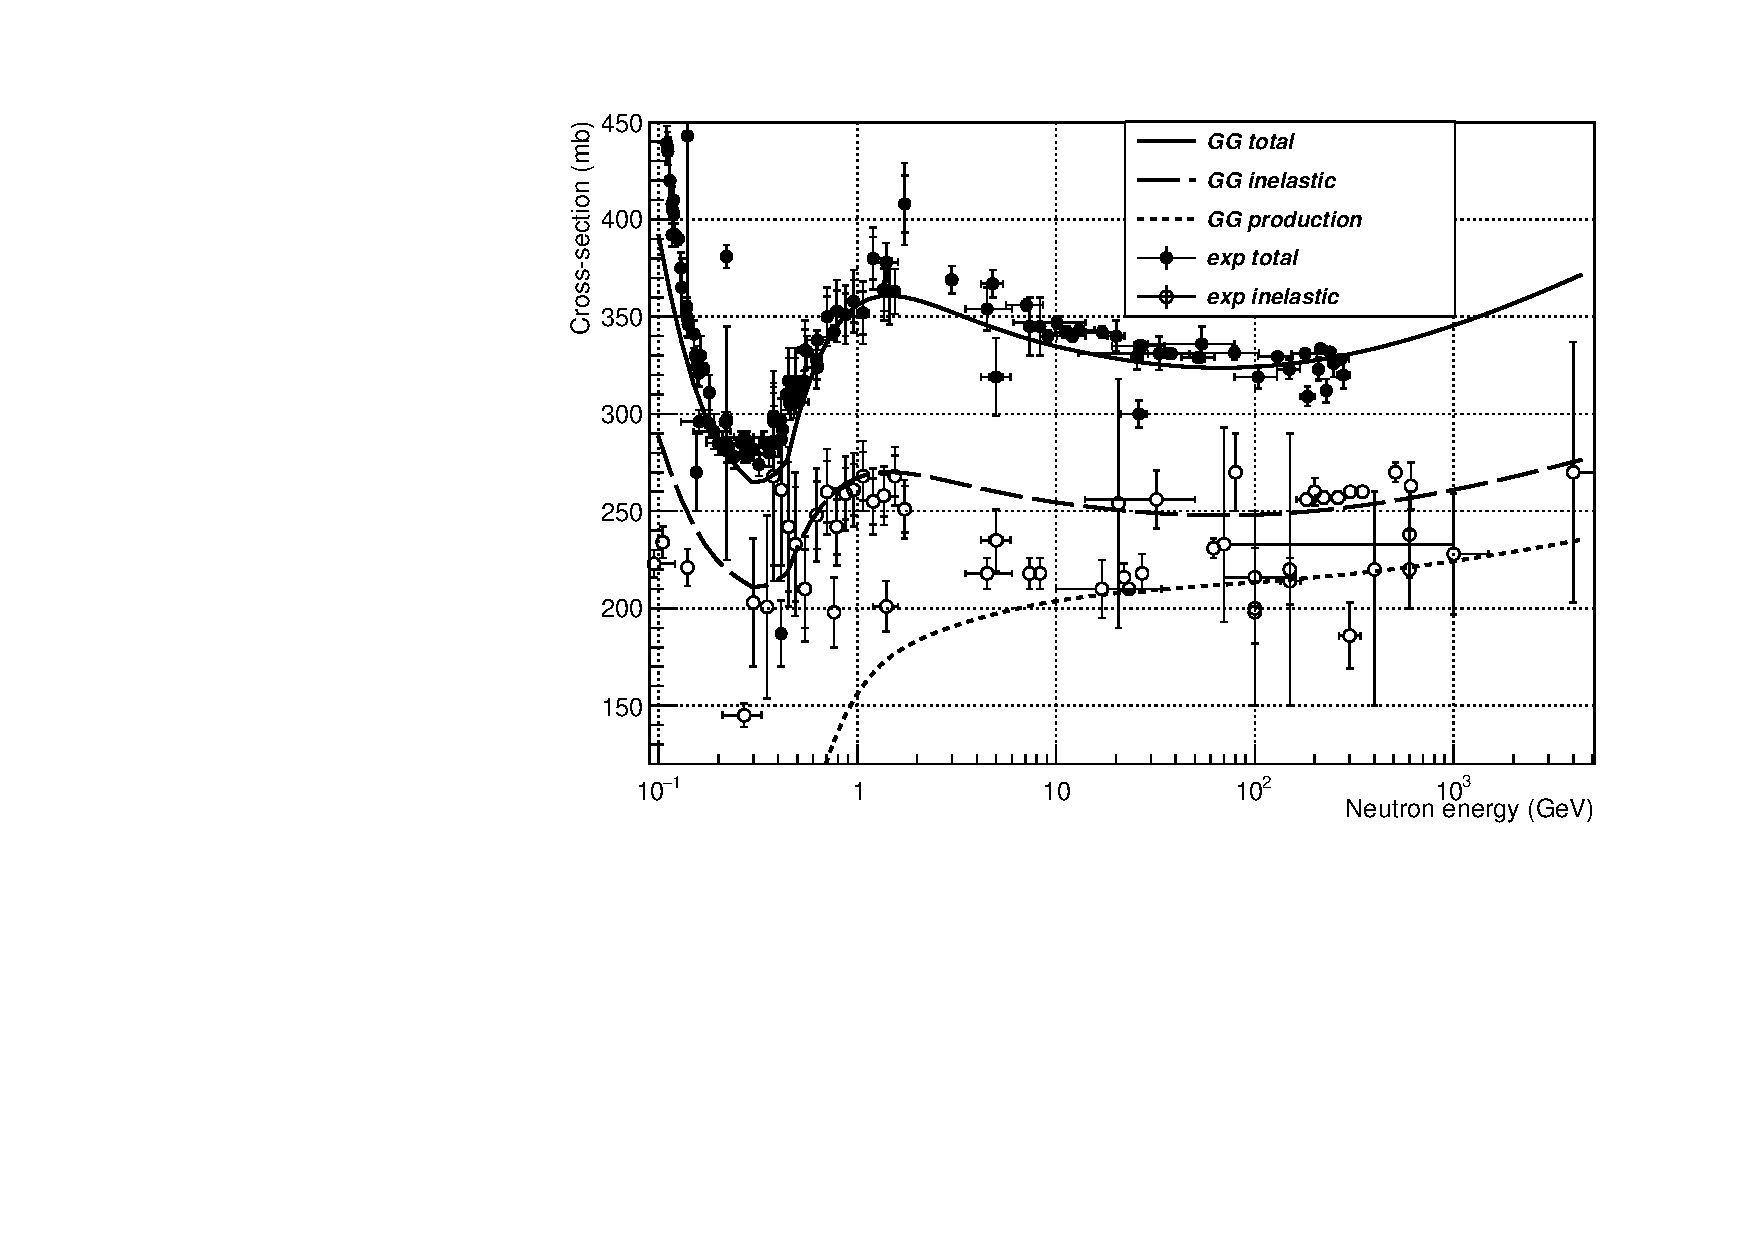
\includegraphics[width=0.5\textwidth]{figures/nCtotinprodGG.pdf}
% \centering \includegraphics[height=3.3in,width=3.6in]{figures/nCtotinprodGG.eps}
\caption{ Total, inelastic and production cross-sections of neutrons on a carbon 
target in the energy range $10^{-2}-10^3$~GeV. Experimental data (open and solid
points) from \cite{hadbib:ihepbase,hadbib:dubnabase}, lines correspond to the 
Glauber-Gribov model.}
\label{nCtotinprodGG}
\end{figure}

\begin{figure}
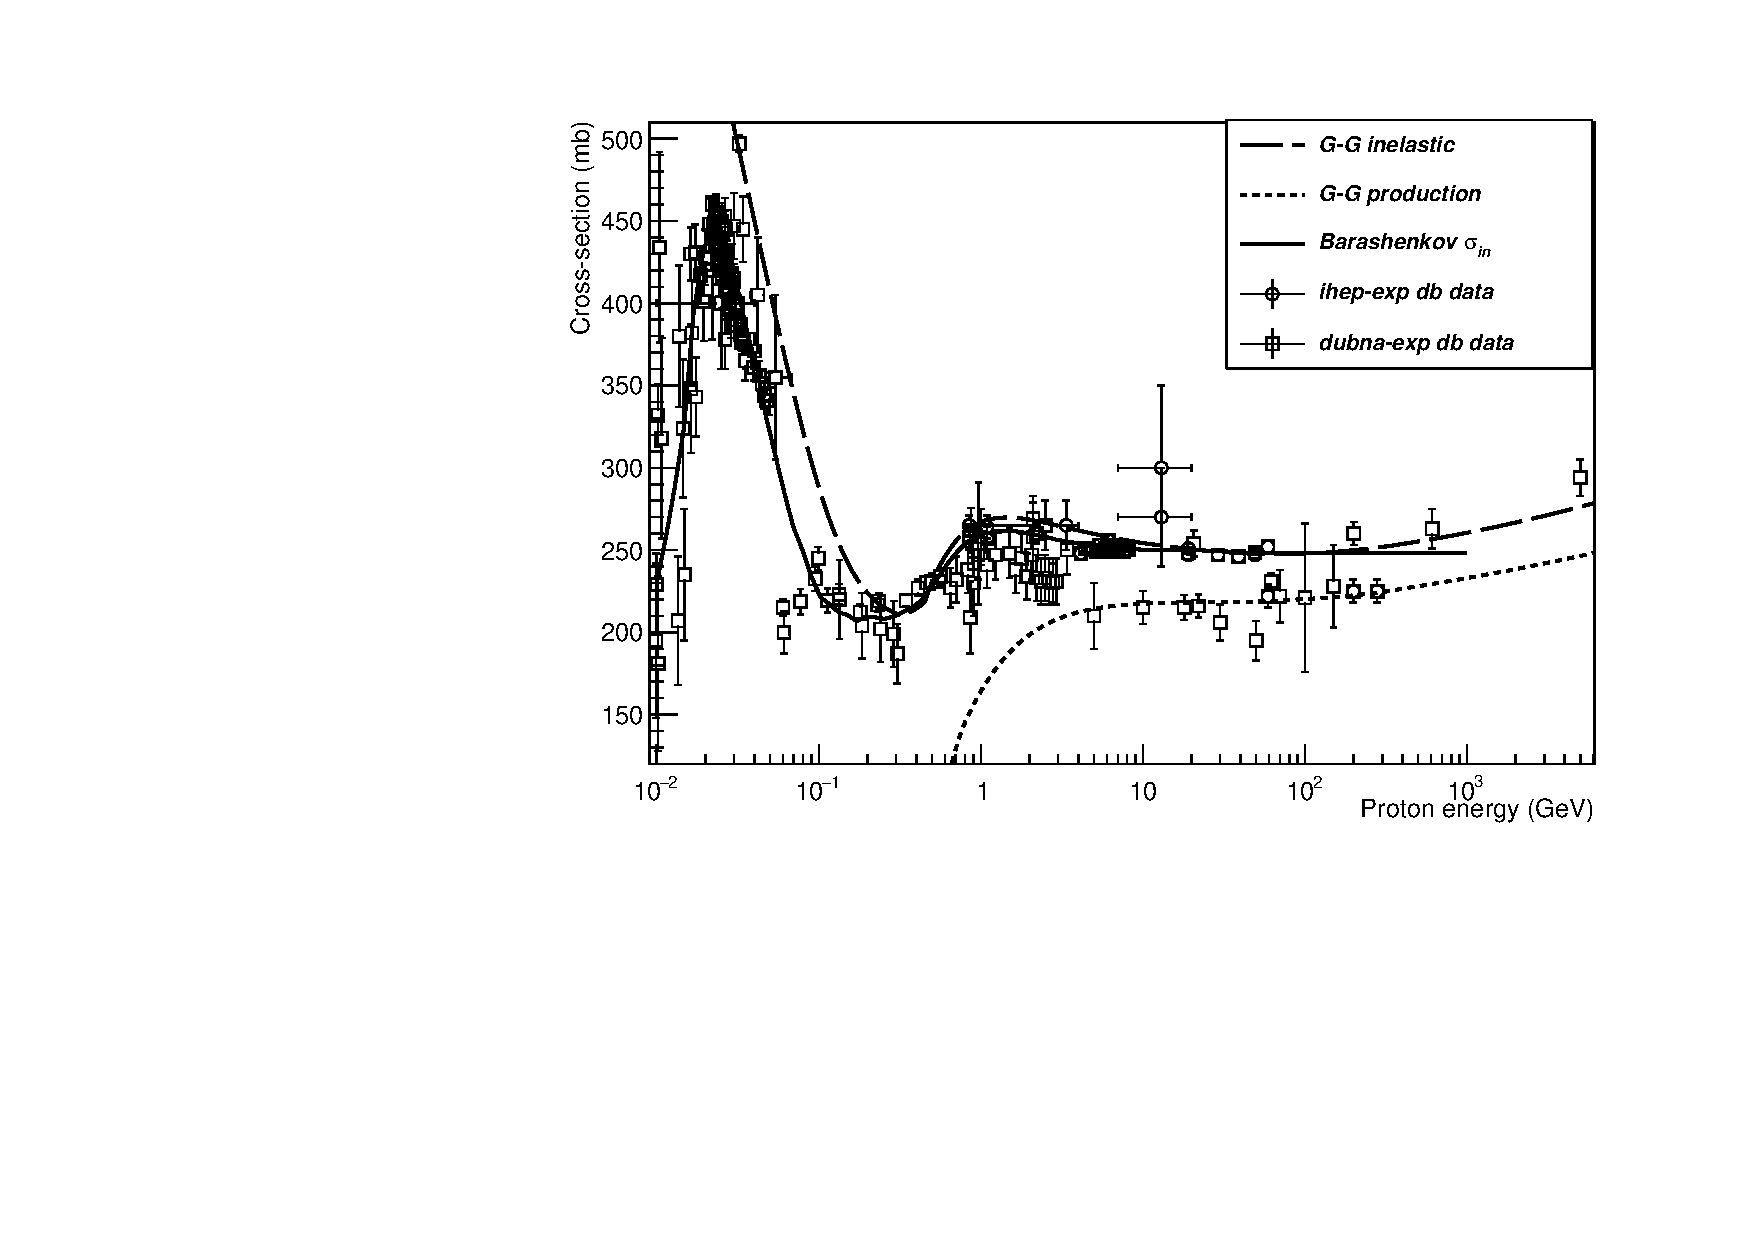
\includegraphics[width=0.5\textwidth]{figures/pCinprodBGG.pdf}
% \centering \includegraphics[height=3.3in,width=3.6in]{figures/pCinprodBGG.eps}
\caption{ Inelastic and production cross-sections of protons on a carbon 
target in the energy range $10^{-2}-10^3$~GeV. Experimental data (open points
and squares) are from \cite{hadbib:ihepbase,hadbib:dubnabase}. The solid and 
dashed lines correspond to the Barashenkov and Glauber-Gribov inelastic models,
respectively.  The dotted line shows the Glauber-Gribov production model.}
\label{pCinprodBGG}
\end{figure}





% done 
%%%%%%%%%%%%%%%%%%%%%%%%%%%%%%%%%%%%%%%%%%%%%%%%%%%
% chipsextract.tex
% Author: Witold Pokorski
%%%%%%%%%%%%%%%%%%%%%%%%%%%%%%%%%%%%%%%%%%%%%%%%%%%
% \noindent {\emph{Extraction of CHIPS kaon and hyperon cross sections}}
\paragraph{Extraction of CHIPS kaon and hyperon cross sections}
The cross sections for kaons and hyperons incident upon nuclei are based on the
parameterization by Kossov and Degtyarenko who developed them as part of the 
CHIPS package \cite{hadbib:CHIPS}.  This parameterization was developed using 
extensive data samples and contains a number of parameters which depend on the
type of projectile.  With \Gfour{} 9.6 these cross sections were made 
independent of the CHIPS package and their interfaces made to conform to the 
hadronic standard in the toolkit.  They are currently used by default in 
production physics lists such as FTFP\_BERT and QGSP\_BERT.



% done
%%%%%%%%%%%%%%%%%%%%%%%%%%%%%%%%%%%%%%%%%%%%%%%%%%%
% antibaryonXS.tex
% Authors: Aida Galoyan, Vladimir Uzhinsky
%%%%%%%%%%%%%%%%%%%%%%%%%%%%%%%%%%%%%%%%%%%%%%%%%%%
%{\bf Anti-baryon Cross Sections} \linebreak[4]
% \noindent {\emph{Antinucleus--nucleus cross sections}}
\paragraph{Antinucleus--nucleus cross sections}
Production of anti-nuclei, especially anti-$^4{\rm He}$, has been observed in
nucleus-nucleus and proton-proton collisions by the RHIC and LHC experiments. 
Contemporary and future experimental studies of anti-nucleus production require
a knowledge of anti-nucleus interaction cross sections with matter which are 
needed to estimate various experimental corrections, especially those due to 
particle losses which reduce the detected rate.  Because only a few measurements
of these cross sections exist, they were calculated using the Glauber approach 
\cite{hadbib:AntiA1,hadbib:AntiA2,hadbib:AntiA3} and the Monte Carlo averaging 
method proposed in \cite{hadbib:AntiA4,hadbib:AntiA5}.

Two main considerations are used in the calculations: a parameterization of the
amplitude of antinucleon-nucleon elastic scattering in the impact parameter
representation and a parameterization of one-particle nuclear densities for
various nuclei. The Gaussian form from \cite{hadbib:AntiA1,hadbib:AntiA3} was
used for the amplitude and for the nuclear density the Woods-Saxon distribution
for intermediate and heavy nuclei and the Gaussian form for light nuclei was 
used, with parameters from the paper \cite{hadbib:AntiA6}. Details of the 
calculations are presented in \cite{hadbib:AntiA7}.

Resulting calculations agree rather well with experimental data on anti-proton
interactions with light and heavy target nuclei ($\chi^2/NoF$ = 258/112) which 
corresponds to an accuracy of $\sim $8\% \cite{hadbib:AntiA7}.  Nearly all
available experimental data were analyzed to get this result.  The predicted 
antideuteron-nucleus cross sections are in agreement with the corresponding 
experimental data \cite{hadbib:AntiA8}.

Direct application of the Glauber approach in software packages like \Gfour{}
is ineffective due to the large number of numerical integrations required. To 
overcome this limitation, a parameterization of calculations 
\cite{hadbib:ggepjc,hadbib:ggnimb} was used, with expressions for the total 
and inelastic cross sections as proposed above in the discussion of the 
Glauber-Gribov extension. Fitting the calculated Glauber cross sections
yields the effective nuclear radii presented in the expressions for $\bar pA$,
$\bar dA$, $\bar tA$ and $\bar \alpha A$ interactions:
\\
$$
R^{eff}_A=a\ A^b\ + \ c/A^{1/3}.
$$
The quantities $a$, $b$ and $c$ are given in \cite{hadbib:AntiA7}.

As a result of these studies, the \Gfour{} toolkit can now simulate 
anti-nucleus interactions with matter for projectiles with momenta between 
100~MeV/c and 1~TeV/c per anti-nucleon.



% done
%%%%%%%%%%%%%%%%%%%%%%%%%%%%%%%%%%%%%%%%%%%%%%%%%%%
% nucleusnucleusXS.tex
% Author: Vladimir Uzhinsky
%%%%%%%%%%%%%%%%%%%%%%%%%%%%%%%%%%%%%%%%%%%%%%%%%%%
\paragraph{Nucleus-nucleus cross sections}
The simulation of nucleus-nucleus interactions and the corresponding cross
sections is required by accelerator experiments, cosmic ray studies and 
medical applications, to name a few domains.

Because nuclei are charged, total and elastic cross sections are
infinite due to Coulomb interaction. In reality, they are restricted
by the screening of the atomic electrons. This interaction leads to a
small-angle scattering which can be ignored in a first approximation.
Thus, inelastic cross sections are the most important ones.
With increasing energy electromagnetic dissociation (EMD) becomes dominant,
especially for the collisions of heavy nuclei.  At low and intermediate energies
EMD does not play an essential role, while the nuclear break-up and 
multi-particle productions dominate.

%{\bf why this sentence is here if we don't use this\\
%There are good methods of EMD calculations
%\cite{hadbib:AAx1,hadbib:AAx2,hadbib:AAx3}, but we do not implement them
%because in low energy domain EMD results mainly in one or two neutron
%production.} 
The strong interaction cross sections can be calculated in the Glauber 
approximation \cite{hadbib:AntiA5,hadbib:AAx4} at high ($>$ 1 GeV) energies.
The description of the cross sections at low and intermediate energies is the
challenging component.

%{\bf All the next section is very confusing, it seems a historical excursus that does not clarify really what is used in G4,
%we should substantially revisit this\\
%Very simple expression was proposed in paper \cite{hadbib:AAx5} many years
%ago -- $\sigma_{AB}=\pi (R_A+R_B-c)^2$, where $R_A$ and $R_B$ are radii of
%$A$ and $B$ nuclei ($R_A=r_0\ A^{1/3}$). As it was found latter,
%$r_0\simeq$ 1.36 fm, and $c\sim$ 0 -- 1.5 fm which depend on a projectile
%energy. In papers \cite{hadbib:AAx6}, the following expression was proposed
%for $c$, $c=x(A^{-1/3}+B^{-1/3})$. It was additional improved in
%the paper \cite{hadbib:AAx7}.

%In order to extend the parameterization in the intermediate energy range,
%authors of the paper \cite{hadbib:AAx8} considered the expression:
%$\sigma_{AB}=\pi R_{int}^2\ (1-B/E_{CMS})$, where $R_{int}$ was subdivided
%into two parts, one was energy independent according to the author's analysis
%of experimental data, the second term had an energy dependence. $B$ is
%the Coulomb barrier of projectile-target system, and $E_{CMS}$ is CMS-energy
%of the system: $B=Z_A Z_B e^2/r_C(A^{1/3}+B^{1/3})$. At this, they obtained
%more reasonable value for $r_0$, $r_0=1.1$ fm. The parameterization was also
%applyed at low energies \cite{hadbib:AAx9} introdicing more parameters, and
%fitting experimental data. Recently, the last parameterization was validated for
%light nucleus projectiles \cite{hadbib:AAx10}. As it was shown there,
%the approach works rather well.\\
%Proposal:\\
%}
A first simple expression was proposed in \cite{hadbib:AAx5}:
$\sigma_{1,2}=\pi (R_1+R_2-c)^2$, where $R_1$ and $R_2$ are the radii of
the two interacting nuclei ($R=r_0\ A^{1/3}$), $r_0\simeq$ 1.36 fm, and 
$c\sim$ 0 -- 1.5 fm, depending on a projectile energy (following  
\cite{hadbib:AAx6} and the further refinements of \cite{hadbib:AAx7}
 $c \propto (A_1^{-1/3}+A_2^{-1/3})$).

In order to extend the parameterization to the intermediate energy range
\cite{hadbib:AAx8} $\sigma_{AB} = \pi R_{int}^2\ (1-B/E_{CMS})$ can be used,
where $R_{int}$ is composed of two terms, energy dependent and independent, 
$B = Z_A Z_B e^2/r_C(A^{1/3}+B^{1/3})$ is the Coulomb barrier of the 
projectile-target system, and $E_{CMS}$ is center-of-mass system energy.

In \Gfour{} the ``Sihver'', ``Kox'' and ``Shen'' parameterizations 
\cite{hadbib:AAx7,hadbib:AAx8,hadbib:AAx9} are used, with the Shen 
parameterization recommended for all physics lists.



\subsubsection{Hadronic models and processes}\label{sec:models}
Due to the large energy range covered, it is not possible for a single model to
describe all the physics encountered in a simulation.  A typical sequence of 
reactions may begin with a high energy hadron-nucleon collision within a nucleus
(QCD or parton string model), followed by the propagation of the secondaries of 
the collision through the nuclear medium (intra-nuclear cascade model), followed
by the de-excitation of the remnant nucleus (precompound model) and its 
evaporation of particles (evaporation and breakup models) until it reaches the 
ground state.  Each of these stages is qualitatively different from the other 
and will be discussed in turn, highlighting recent developments. 

Other reactions covered include nucleus-nucleus interactions (QMD or 
parton-based models), elastic models  (including coherent hadron scattering 
from nuclei), capture, and lepton- and gamma-nuclear interactions.

% Some of them are considered in
% Sec.~\ref{sec:models}. At low energy ($<$ 10 MeV) a negative charged or neutral
% particle can be absorbed by a target nucleus. A simulation of the reactions
% is presented in subsection~\ref{had:stopping}. At higher energies but below
% meson production threshold there can be only elastic hadron-nucleon scattering
% and potential interactions.
% Thus we have implemented in \Gfour three of
% such models -- BIN, QMD and \inclxx. The binary model (BIN) was described in
% \Gfour paper~\cite{G4}. Below a short description of the QMD model and
% the Li\`{e}ge Intranuclear Cascade model (\inclxx) will be presented
% \cite{hadbib:inclxx}.

%%%%%%%%%%%%%%%%%%%%%%%%%%%%%%%%%%%%%%%%%%%%%%%%%%%%%%%%%%
% string.tex
% Authors: Alberto Ribon, Vladimir Uzhinsky, Gunter Folger
%%%%%%%%%%%%%%%%%%%%%%%%%%%%%%%%%%%%%%%%%%%%%%%%%%%%%%%%%%
\paragraph{Quark-gluon string models}
Two models based on quark-parton concepts were implemented in \Gfour{}, the
Quark-Gluon String (QGS) model
% proposed by A. Capella and A.B. Kaidalov
\cite{hadbib:FTF1,hadbib:FTF2} and the Fritiof (FTF) model.
% by Andersson et al.
\cite{hadbib:FTF3,hadbib:FTF4}.
The QGS model is described in \cite{bib:G4}.  A short description of the FTF
model is presented here, but more details are available in the \Gfour{} 
Physics Reference Manual \cite{hadbib:FTF19}.

%of the FTF model will be presented which is
%in production PhysicsLists of \Gfour used by LHC experiments.

The FTF model is used in \Gfour{} to simulate the following interactions:
hadron-nucleus at incident laboratory hadron momenta $>$ 3--5 GeV/c, 
nucleus-nucleus at incident laboratory hadron momenta $>$ 2--3 GeV/c/nucleon,
antibaryon-nucleus at all energies, and antinucleus-nucleus.
Because the model does not include multi-jet production in hadron-nucleon 
interactions, the upper limit of its validity range is estimated to be 1~TeV/c 
per hadron.

The modeling of hadron-nucleon interactions in the FTF model includes the
simulation of elastic scattering, binary reactions such as 
$NN\rightarrow N\Delta$ and $\pi N\rightarrow \pi \Delta$, single diffractive 
and non-diffractive events, and annihilation in anti-baryon-nucleon interactions.
Interactions proceed by the production of one or two unstable objects called 
quark-gluon strings.  If only one string is created, the process is called 
diffraction dissociation.  

In the \Gfour{} implementation single diffraction dissociation is simulated 
separately from non-diffractive interactions.  A special function which 
corresponds to a weighted simulation of the diffraction dissociation was
introduced to perform this separation.  In most other Fritiof-based models 
this separation is governed by a single parameter, which is not sufficient for
a correct description of the large set of experimental data. 

Once formed, strings may interact with other nucleons in hadron-nucleus and 
nucleus-nucleus collisions, producing additional strings.  Strings with 
sufficiently large mass ($>$ 1.2~GeV) may in general have kinks, which are
treated as emitted gluons which decay into quark-antiquark pairs.  This feature
is required in order to reproduce particle multiplicities observed in hadronic 
interactions at high energies.  However, the current FTF implmentation does not 
handle kinks, hence the TeV/c upper limit.  

% Because multi-gluon production in elementary interactions is
% not included in FTF, the upper limit of the model's validity is estimated to be 
% 1~TeV, sufficient for most applications of \Gfour{}.

Hadron-nucleon scattering within the model uses the elastic and inelastic cross 
sections taken from the CHIPS parameterizations \cite{hadbib:CHIPS}. 
Cross sections for binary reactions and diffraction dissociation were implemented
directly in the FTF model as parameterizations of data.  Here the cross sections
for the unstable objects were taken to be the same as those for stable objects
with the same quark content.  

Once the unstable objects are produced, the LUND string fragmentation model is 
used to decay them \cite{hadbib:FTF7}.  The parameters of this model were tuned
to experimental data and the available phase space was restricted to take into 
account low mass string fragmentation.  The formation time of hadrons was also 
applied.

To simulate hadron-nucleus and nucleus-nucleus scattering it is necessary to 
embed the hadron-nucleon interaction in the nuclear environment.  This was done
by first assuming a Woods-Saxon parameterization of the one-particle nuclear 
density for medium and heavy nuclei and a harmonic oscillator shape for light 
nuclei.  Center-of-mass correlations and short-range nucleon-nucleon 
correlations were taken into account.  A simplified Glauber model was used to 
sample the multiplicity of intra-nuclear collisions.  Screening was not 
considered; estimates and data indicate that it decreases the total 
hadron-nucleus cross sections by 3--5\%, while the inelastic hadron-nucleus 
cross sections are practically unchanged \cite{hadbib:Alvi}.  Hence any effect 
on the multiplicity of produced particles is expected to be small.

The number of string objects in non-diffractive interactions is proportional to
the number of participating nucleons. Thus, multiplicities in hadron-nucleus and
nucleus-nucleus interactions are larger than those in elementary interactions.
It is assumed that the reaction creating unstable strings in hadron-nucleus
collisions is analogous to that in nucleus-nucleus collisions.

It is known that the Glauber approximation used in this and other string models
does not provide enough intra-nuclear collisions for a correct description of
nuclear destruction.  Traditional cascade models would fulfill this need, except 
that they produce too many particles.  Reggeon theory has been proposed to solve
this problem \cite{hadbib:FTF18}, but the detailed calculation required was not
appropriate for a reasonably fast computer code.  A simplified implementation in
\Gfour{} assumes \cite{hadbib:FTF10} that participating nucleons predicted by the 
Glauber approximation initiate low energy reggeon exchanges in the spectator 
part of a target nucleus.  This reggeon theory inspired model (RTIM) provides 
the right number of fast nucleons ejected during nuclear destruction and 
describes secondary particle intra-nuclear cascading \cite{hadbib:FTF8}.   

The collective nature of nuclear destruction led to the introduction of a new
"Fermi motion" \cite{hadbib:FTF9,hadbib:FTF10} simulation which is a refined 
algorithm for putting involved nucleons on the mass-shell.  As shown in 
Figure~\ref{had:FTFfig1}, this provides sufficient agreement with experimental
data in the transition region, around 3~GeV/c.

When the cascading is finished, the excitation energies of residual nuclei are
estimated in the ``wounded nucleon'' approximation \cite{hadbib:FTF11}. This 
allows for a direct coupling of the FTF model to the \Gfour{} precompound model
and its nuclear fragmentation sub-models.  The determination of the particle
formation time also allows coupling of the FTF model to the \Gfour{} Binary 
cascade model \cite{hadbib:FTF12}.

%The Ultra-Relativistic Quantum Molecular Dynamic model (UrQMD) \cite{hadbib:FTF13}
%simulates the binary reactions, but it seems to as that their cross sections are
%not tuned quite well. 

% An effort is underway to fit the cross sections in the FTF model, but up to
% now only low mass resonances have been considered. It is thus expected that the
% FTF model is not entirely correct at projectile energies below 3--5 GeV.

% A peculiarity of the \Gfour Fritiof model implementation is the separate 
% simulation of the single diffraction dissociation and non-diffractive 
% interactions. In most Fritiof-based models the separation between the processes
% is governed by a single parameter.  This, however, is not sufficient for a 
% correct description of the large set of experimental data.  A special function
% for this separation was therefore introduced, which corresponds to a weighted 
% simulation of the diffraction dissociation.

Two additional innovations were made in the FTF model, one dealing with low-mass
strings and the other making multiplicity corrections in hadron-nucleus and
nucleus-nucleus reactions.
   
All Monte Carlo event generators are challenged with the correct treatment 
of low mass strings. Such a string is typically handled by first checking that
it can decay into two low mass particles. If it can, the decay is simulated;
otherwise, the string is converted into a hadron.  This step violates 
energy-momentum conservation and the momenta of all other produced particles
must be adjusted to correct for this.  In the FTF model all strings with 
sufficiently large mass are allowed to decay to two particles.  As a result, the
cross sections of the reactions $\bar p+p \rightarrow \bar n+n$, 
$\bar p+p \rightarrow \bar \Lambda+\Lambda$, and so on, are reproduced. In the 
case of a two-particle decay, all possible final states are considered, and one 
is chosen according to its phase space volume. For other final states, standard 
string fragmentation or direct production of a hadron is possible.  

% Strings with sufficiently large mass ($>$ 1.2 GeV) can have a kink. The kink is
% treated as a gluon which decays into a quark-antiquark pair. This is needed
% to reproduce particle multiplicities observed in hadronic interactions. The 
% UrQMD model \cite{hadbib:FTF13}, for example, does not consider kinky strings,
% while the Hijing model \cite{hadbib:FTF14} assumes copious gluon production in 
% hard and semi-hard interactions. The Fritiof 7.0 model \cite{hadbib:FTF15} also
% considers gluon production. Because multi-gluon production in elementary 
% interactions is not included in the \Gfour FTF model, its upper limit of 
% application is estimated to be 1 TeV, sufficient for most applications of \Gfour.

Multiplicity corrections in hadron-nucleus and nucleus-nucleus interactions are 
necessary when computing the number $N_{bin}$ of intra-nuclear collisions.  The
distribution of $N_{bin}$ is usually obtained by applying the asymptotic AGK 
cutting rules \cite{hadbib:FTF16} to the Glauber amplitude for elastic 
scattering.  These rules must be corrected for finite energies. Because there is
no defined prescription for making these corrections, a phenomenological 
approach, taking into account formation time and using HARP-CDP data 
\cite{hadbib:FTF17}, was adopted.

%{\bf suggest to remove all this and quote an article with details:\\
%As known, a simple cascade model considers only pions and nucleons. Due to this
%it cannot work when resonance production is a dominating process in hadronic
%interactions. But if the energy is sufficiently low the resonances can decay
%before a next possible collision, and the model can be valid.
%  OK above ??
% Let $p$ be the momentum
%of a produced resonance ($\Delta$). The average life time of the resonance in
%its rest frame is $1/\Gamma$. In the laboratory frame the time is
%$E_\Delta/\Gamma m_\Delta$. During this time, the resonance will fly a distance
%$\bar{l}=v\ E_\Delta/\Gamma m_\Delta=p/\Gamma m_\Delta$. If the distance is less
%than an average distance between nucleons in nuclei ($\bar{d}\sim 2$ fm),
%the model can be applied. From the condition, we have:
%$
%p\leq \bar{d}\ \Gamma m_\Delta \sim 1.5
%$
%(GeV/c).
%
%Direct $\Delta$-resonance production takes place in $\pi N$ interactions at low energies.
%Thus the model cannot work well at a momentum of pions above 2 GeV/c. In nucleon-nucleon
%interactions, due to momentum transfer to a target nucleon, the boundary can be higher.
%
%Returning back to the FTF model, let us assume that projectile originated strings
%have an average life time $1/\Gamma$, and an average mass $m^*$. The strings can
%interact on average with $\bar{l}/\bar{d}=p/\Gamma m^*\bar{d}=p/p_0$ nucleons.
%Here $p_0$ is a new parameter. According to our estimates it is about 2 -- 3 GeV/c.
%Thus, we can assume that at any energy there is a maximum number of intra-nuclear
%collisions in the FTF model -- $\nu_{max}=p/p_0$.
%This restriction is implemented in the current version of the FTF model, and puts
%a low boundary of the model application region to 3--5 GeV/c. For the determination
%of the $p_0$ parameter we used the HARP-CDP data \cite{hadbib:FTF17}.
%
%As known, the Glauber approximation used in the Fritiof model and in the other
%string models does not provide enough intra-nuclear collisions for a correct
%description of a nuclear destruction. Additional cascading in nuclei is needed!
%Usage of a standard cascade for secondary particle interactions leads to a large
%multiplicity of produced particles. Usually, it is assumed that an inclusion of
%a secondary particle's formation time can help to solve this problem, but there
%is no unified solution. The concept of the formation time was criticized in
%the paper \cite{hadbib:FTF18} where the intra-nuclear cascade was considered
%from the reggeon theory point of view. Because we were not be able to implement
%a complicated reggeon calculation scheme, we have assumed \cite{hadbib:FTF10}
%that participating nucleons predicted by the Glauber approximation initiate
%low energy reggeon exchanges in a spectator part of a target nucleus (reggeon
%cascading). This provide us with an enough amount of fast nucleons ejected at
%a target nucleus destruction.
%
% This collective nature of the destruction
%pushed us to introduce a new "Fermi motion" simulation which is a refined
%algorithm of putting of involved nucleons onto mass-shell.  All of these
%allowed us to obtain a smooth transition from the FTF model and low energy
%Bertini and Binary cascade models of \Gfour (see Fig.~\ref{had:FTFfig1}a).
%
%The main problem now is an accounting of the diffraction dissociation in
%hadron-nucleus and nucleus-nucleus interactions. A transition of a projectile
%particles into a diffractive system and back during elastic scattering on a nucleus
%has to be suppressed by the nuclear form-factor. Due to this a projectile
%diffraction dissociation in inelastic interactions has to be also suppressed
%according to the reggeon phenomenology. One cannot apply this consideration
%to a target nucleon diffraction, and one can assume that they can dissociate.
%But the calculations presented in Fig.~\ref{had:FTFfig1} were done without
%the suppression for $p{\rm Ta}$ interactions, and with full suppression for
%$\pi {\rm Ta}$ interactions. Another choice makes the description worse.
%The question is now under the study.
%}

\begin{figure}
\centering
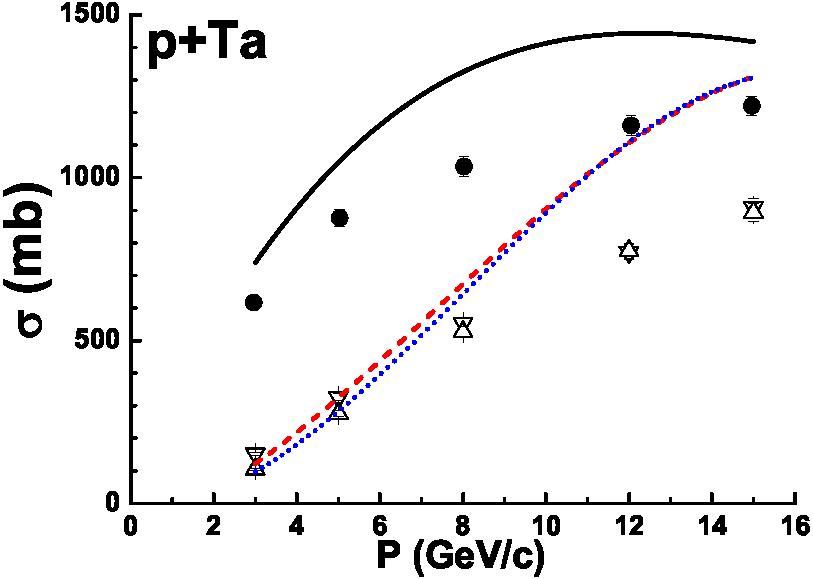
\includegraphics[height=1.8in,width=1.70in]{figures/FTFfig1_1.pdf}
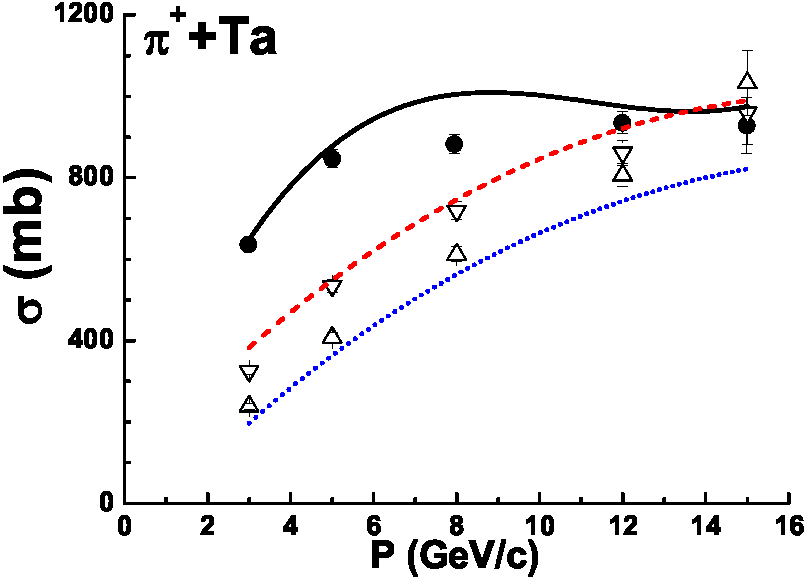
\includegraphics[height=1.8in,width=1.7in]{figures/FTFfig1_2.pdf}
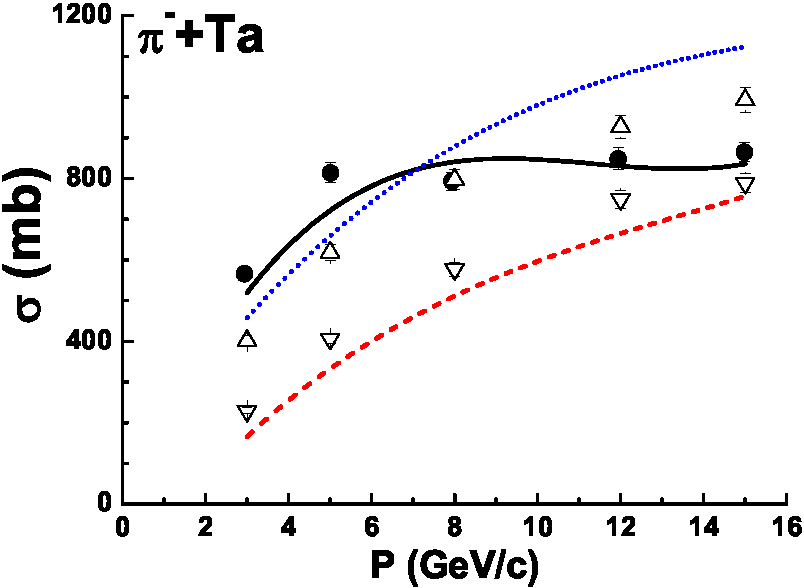
\includegraphics[height=1.8in,width=1.7in]{figures/FTFfig1_3.pdf}
\caption{Inclusive cross sections for $p$, $\pi^+$ and $\pi^-$ production in
         $p{\rm Ta}$, $\pi^+{\rm Ta}$ and $\pi^-{\rm Ta}$ interactions as a 
         function of projectile hadron momentum.  Data from the HARP-CDP 
         group \protect{\cite{hadbib:FTF17}} are shown as closed circles for
         protons and up- and down-triangles for $\pi^+$ and $\pi^-$,
         respectively.  Lines are FTF model calculations: solid for protons,
         dashed and short-dashed for $\pi^+$ and $\pi^-$, respectively.}
\label{had:FTFfig1}
\end{figure}


  \label{had:string}
%%%%%%%%%%%%%%%%%%%%%%%%%%%%%%%%%%%%%%%%%%%%%%%%%%%%%%%%%%%%%%%%%%%%
% cascade.tex
% Authors: Mike Kelsey, Davide Mancusi, Gunter Folger, Dennis Wright
%%%%%%%%%%%%%%%%%%%%%%%%%%%%%%%%%%%%%%%%%%%%%%%%%%%%%%%%%%%%%%%%%%%%
\paragraph{Intranuclear cascade models}
% \noindent {\emph{Intranuclear cascade models}}
Three intranuclear cascade models are now offered in \Gfour{}: Bertini, Binary
and INCL++.  The extended Bertini cascade \cite{hadbib:bert} is valid for
p, n, $\pi$, K, $\Lambda$, $\Sigma$, $\Xi$, $\Omega$ and $\gamma$ projectiles
with incident energies between 0 and 15 GeV.  It is also valid for captured 
$\mu^-$ , $K^-$ and $\Sigma^-$.  Recent extensions allow this model to be used
for cascades initiated by high energy muons and electrons.  Although this model
has its own precompound and deexcitation code, an option exists for using the 
native \Gfour{} precompound and deexcitation modules discussed in the following
section.
%  \cite{hadbib:pnst-preco-2011}.

The Binary cascade \cite{hadbib:binary} simulates p and n-induced cascades
below 10 GeV, and $\pi$-induced cascades below 1.3 GeV.  This is done by 
propagating hadrons in a smooth nuclear potential, and forming and decaying 
strong resonances to produce secondaries.  The model relies on the native 
\Gfour{} precompound and deexcitation code to handle the post-cascade steps. 

The Li\`ege Intranuclear Cascade model (\incl) \cite{hadbib:incl} has seen
extensive development since its introduction in \Gfour{}. The original Fortran 
model was completely redesigned and rewritten in C++ and is now known as 
\inclxx\ \cite{hadbib:inclxx}. It extends the applicability of the legacy 
version up to $\sim15$~GeV incident energy, while remaining physics-wise 
equivalent for nucleon- and pion-induced reactions below 1~GeV. In addition,
\inclxx\ has been extended to handle reactions induced by light ions up to
$A=18$.  By default, \inclxx\ uses the \Gfour{} native de-excitation immediately
after the cascade stage; it does not include an intermediate pre-equilibrium 
step.  Coupling to the \abla\ de-excitation model \cite{hadbib:ablav3} is also
possible.

% Quesada, J.M., Ivantchenko V., Ivantchenko A., Cortes M.A., Folger G.,
% Howard A., Wright D. Recent Developments in Pre-Equilibrium and 
% De-excitation Models in Geant4. Progress in Nuclear Science and Technology. 
% Proceedings of the Joint International Conference Supercomputing in Nuclear 
% Applications and Monte Carlo 2010. October 17-21. Tokyo, Japan.
 \label{had:cascade}
%%%%%%%%%%%%%%%%%%%%%%%%%%%%%%%%%%%%%%%%%%%%%%%%%%%
% precompound.tex
% Author: Jose-Manuel Quesada
%%%%%%%%%%%%%%%%%%%%%%%%%%%%%%%%%%%%%%%%%%%%%%%%%%%
\paragraph{The precompound model}
The native \Gfour{} pre-equilibrium  model is based on a version of the 
semi-classical exciton model \cite{hadbib:gudima83} and is used as the back-end
stage of several cascade and quark-gluon string generators.  It handles the 
de-excitation of the remnant nucleus from its formation immediately following a
cascade or high energy collision, until it reaches equilibrium.  During this 
time, internal transitions of the pre-compound nuclear system compete with 
nucleon and light cluster emissions.  The passage to the state of statistical 
equilibrium, which happens when the transition probabilities for increasing and 
decreasing the exciton number become approximately equal (equilibrium condition),
is roughly characterized by an equilibrium number of excitons $n_{eq}$.  In the
simulation $n_{eq}$ is a calculated number based on the assumption that the 
equilibrium condition is met. 

Some refinements were introduced recently 
\cite{hadbib:calor-2008, hadbib:ijrb-space-2012, hadbib:iaea-spa-2009}, 
namely more realistic inverse cross section parameterizations and combinatorial
factors for particle emission, a phenomenological parameterization of the 
transition matrix elements, and a more physically consistent condition for the 
transition to equilibrium, since in certain circumstances this condition is 
reached well before the previously used rough estimate of $n_{eq}$.

At the end of the pre-equilibrium stage, the residual nucleus should be left in
an equilibrium state, in which the excitation energy is shared by the entire 
nuclear system.  Such an equilibrated compound nucleus is characterized by its 
mass, charge and excitation energy with no further memory of the steps which led
to its formation.

 
%%%%%%%%%%%%%%%%%%%%%%%%%%%%%%%%%%%%%%%%%%%%%%%%%%%%%%%%%%%%%%%%%%%
% deexcitation.tex
% Authors: Vladimir Ivantchenko, Jose Manuel Quesada, Gunter Folger
%%%%%%%%%%%%%%%%%%%%%%%%%%%%%%%%%%%%%%%%%%%%%%%%%%%%%%%%%%%%%%%%%%%
\paragraph{Nuclear de-excitation models}
The final de-excitation of a nucleus to a thermalized state is simulated by
several semi-classical models which are responsible for sampling the 
multiplicity of neutrons, protons, light ions, isotopes, and photons.  They
are:
\begin{itemize}
\item Fermi break-up (FBU) \cite{hadbib:mfm-bondorf-1995},
\item statistical multifragmentation \cite{hadbib:mfm-bondorf-1995},
\item fission, based on the Bohr-Wheeler semi-classical model 
      \cite{hadbib:jinr-fis-1977, hadbib:inr-fis-1993},
\item evaporation of nucleons and light fragments, which is handled by models 
      based on either
\begin{itemize}
  \item the Weisskopf-Ewing model \cite{hadbib:weisskopf-1940} for fragments up
        to and including $\alpha$ particles, or
  \item the generalized evaporation model (GEM) \cite{hadbib:gem-2001} for the 
        emission of fragments with masses up to $^{28}$Mg, and 
\end{itemize}
\item \gclass{G4PhotonEvaporation}, which simulates the emission of  
\begin{itemize}
\item discrete gammas according to the E1, M1 and E2 transition probabilities
      taken from the PhotonEvaporation database, which in turn is based on 
      the Evaluated Nuclear Structure Data File (ENSDF) \cite{hadbib:ENSDF}, 
      and 
\item continuous gammas according to the E1 giant dipole resonance strength 
      distribution.
\end{itemize}
\end{itemize}

These models are managed by the \gclass{G4ExcitationHandler} class, in which
they may be invoked in complement or sometimes concurrently with each other.
Some of them have been thoroughly validated and have undergone continuous 
improvement in recent years \cite{hadbib:calor-2008, hadbib:pmb-fluka-g4-2011}.

In order to properly describe the double differential cross sections and isotope
production data of the IAEA spallation benchmark 
\cite{hadbib-iaea-spa-benchmark,hadbib:iaea-spa-2009}, the standard and GEM 
models were combined to form a hybrid model, and the fission model was improved
\cite{hadbib:pnst-preco-2011,hadbib:ijrb-space-2012,hadbib:iaea-spa-2009}.

For radiobiological applications it is essential that the FBU model be used by 
default for the de-excitation of light fragments (Z $<$ 9, A $<$ 17), taking 
into account Pauli blocking and all possible decay channels into stable and 
long-lived fragments.  Validations
\cite{hadbib:nima-pshenich-2010,hadbib:pmb-fluka-g4-2011}
triggered many of the refinements to this model.

For proton and ion beam therapy applications, the photon evaporation model, 
which is critical for the tracking of the Bragg peak from emitted prompt gammas, 
was improved \cite{hadbib:prompt-gamma-2014}.  The statistical 
multifragmentation model, responsible for the explosive break-up of heavier hot
nuclei  (Z $>$ 8, A $>$ 16, and excitation energy $>$ 3 MeV/u), is relevant 
in simulations of shielding from cosmic radiation and has also been validated
\cite{hadbib:ijrb-space-2012,hadbib:nima-pshenich-2010}. 

 \label{had:deexcitation}

%%%%%%%%%%%%%%%%%%%%%%%%%%%%%%%%%%%%%%%%%%%%%%%%%%%%%%%%%%%%%%%%%
% elastic.tex
% Authors: Vladimir Ivantchenko, Vladimir Grichine, Dennis Wright
%%%%%%%%%%%%%%%%%%%%%%%%%%%%%%%%%%%%%%%%%%%%%%%%%%%%%%%%%%%%%%%%%
\paragraph{Elastic scattering models}
Four options exist in \Gfour{} for the simulation of elastic hadron scattering
from nuclei: the GHEISHA-based and CHIPS-based parameterized models,
the Glauber approach, and diffuse diffraction.

The GHEISHA-based models (\gclass{G4HadronElastic}) \cite{hadbib:gheisha} are
valid for all long-lived hadrons at all incident energies.  They sample the 
momentum transfer from a sum of exponentials whose amplitudes are parameterized
in $Z$, $A$ and incident momentum.  These models are fast, but significantly 
overshoot the data at large angles.

The CHIPS-based models (\gclass{G4ChipsElasticModel}) \cite{hadbib:CHIPS} are
similar, but sample the momentum transfer from a more complex parameterization
which includes details of the nuclear size and potential.  Hence, features like 
diffraction minima are represented.  This model is valid for incident protons,
neutrons, pions, kaons and anti-protons at all energies.

The \gclass{G4ElasticHadrNucleusHE} model depends on Glauber multiple scattering
\cite{hadbib:glauber70} in a nucleus which is described by its impact parameter 
profile.  The energy dependence of the scattering is largely determined by a 
phenomenological combination of hadron-nucleon cross sections.  The model is
valid for all long-lived hadrons of energies greater than 1 GeV.

The \gclass{G4DiffuseElastic} model \cite{hadbib:difel} uses an optical model
of the nucleus and takes into account the diffuse nuclear halo as well as Coulomb 
effects.  It is valid for incident protons, neutrons, pions and kaons of all 
energies.    

The four models are compared to data for 1 GeV protons on silicon in 
Figure~\ref{pSiT1GeVmodsum}.

\begin{figure}
% \centering \includegraphics[height=3.3in,width=3.6in]{figures/pSiT1GeVmodsum.eps}
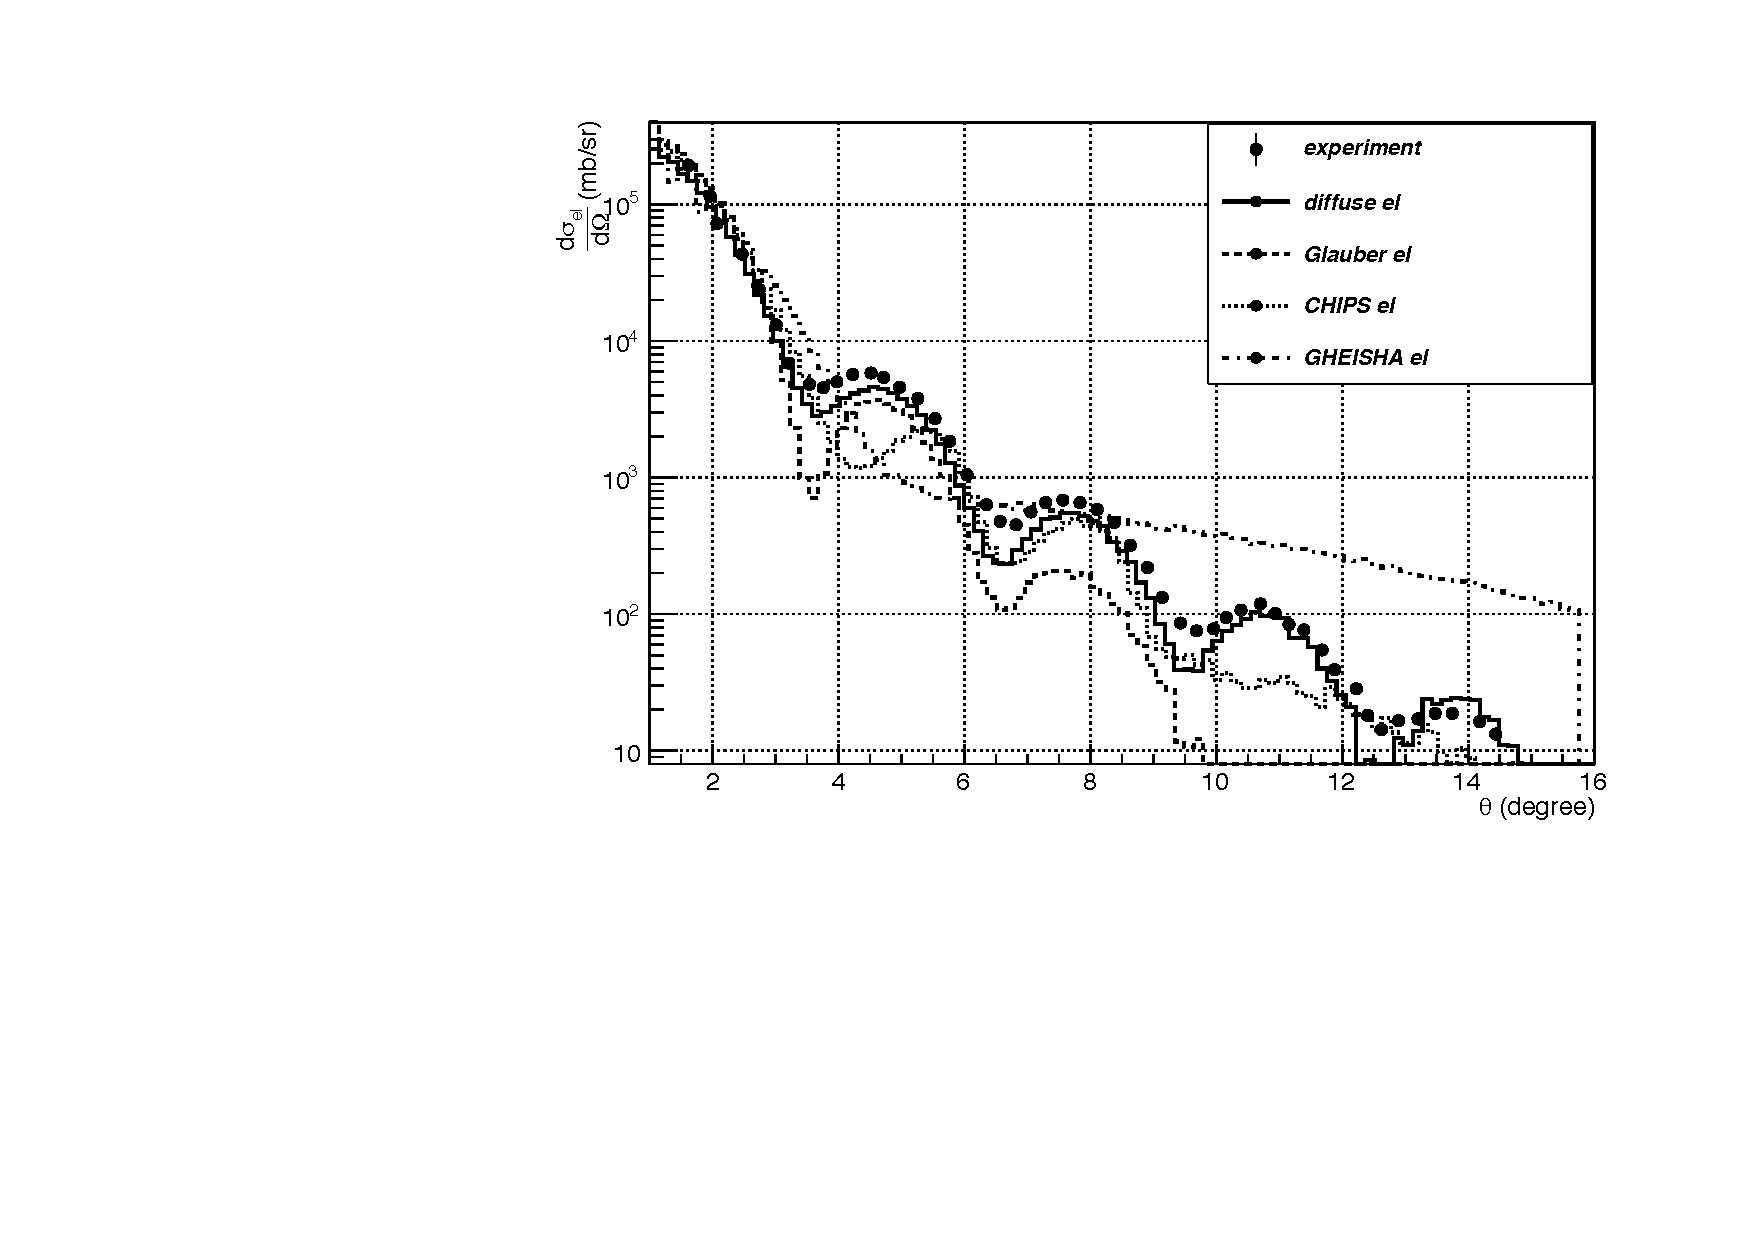
\includegraphics[width=0.5\textwidth]{figures/pSiT1GeVmodsum.pdf}
\caption{Differential elastic scattering cross sections for 1 GeV protons on 
         silicon versus polar scattering angle.  The histograms represent the 
         diffuse, Glauber, CHIPS and GHEISHA models. The solid circles are 
         experimental data~\cite{hadbib:alkh78}.}
\label{pSiT1GeVmodsum}
\end{figure}




%%%%%%%%%%%%%%%%%%%%%%%%%%%%%%%%%%%%%%%%%%%%%%%%%%%
% stopping.tex
% Authors: Julia Yarba, Mike Kelsey, Krzysztof Genser
%%%%%%%%%%%%%%%%%%%%%%%%%%%%%%%%%%%%%%%%%%%%%%%%%%%
\paragraph{Stopping models}
The \Gfour{} toolkit includes processes to simulate the stopping and capture of
hadrons and heavy leptons on nuclei.  Previous parameterized models for $\pi^-$
and $K^-$ capture were replaced by the \Gfour{} Bertini intranuclear cascade for 
negative mesons, baryons and muons, and with the FTF string model for antibaryon
capture and annihilation.  

The Bertini cascade model handles the capture process by selecting a random
location within the nucleus, weighted by the radial nucelon density, to initiate
the cascade process.  The subsequent cascade is propagated using the same code 
used for any other hadron-nucleus interaction.  In the FTF model, the antibaryon
annihilates with a nucleon near the outer ``surface'' of the nucleus, producing 
a small number of pions.  Those secondaries and the excited nucleus are passed 
either to the \Gfour{} de-excitation model (invoked by \gclass{G4PrecompoundModel}),
or to one of the cascade models (Bertini or Binary) for final disposition 
depending on the energy.

Capture of negative muons on nuclei is also handled using the Bertini model.
The muon capture process deals with the atomic capture, the subsequent 
electromagnetic cascade of the muon down to the lowest orbit, including
photon and Auger electron emissions, and the decision about whether the
bound muon should decay in that orbit or be captured into the nucleus.  If
the latter, the Bertini cascade selects a random location within the nucleus 
(weighted as above), where the $\mu^-$ interacts with a proton, producing a 
neutron, neutrino, and one or more radiative photons.  Note that in \Gfour{} 
release 10.0 onward, the radiative cross sections have been set to zero.  As 
above, the neutron is treated as a cascade secondary and processed using the 
existing code of the Bertini model.

 \label{had:stopping}

% needs names of kinematic models 
%%%%%%%%%%%%%%%%%%%%%%%%%%%%%%%%%%%%%%%%%%%%%%%%%%%
% neutrons.tex
% Authors: Tatsumi Koi, Vladimir Ivantchenko
%%%%%%%%%%%%%%%%%%%%%%%%%%%%%%%%%%%%%%%%%%%%%%%%%%%
\paragraph{Low energy neutron models}
As of \Gfour{} 10.0, there were three models treating low energy neutrons with
high precision: NeutronHP, LEND and NeutronXS.  The NeutronHP models, for
elastic, inelastic, capture and fission reactions, have been part of \Gfour{}
for many years \cite{bib:G4}.  They depend on the \Gfour{} Neutron Data Library 
(G4NDL) for cross sections, branching ratios, final state multiplicities and
final state energy and angular distribution parameters.  In its original 
formulation, G4NDL data were drawn from nine different databases,
ENDF/B-VI \cite{hadbib:ENDF}, Brond-2.1 \cite{hadbib:BROND}, CENDL2.2
\cite{hadbib:CENDL}, EFF-3 \cite{hadbib:EFF}, FENDL/E2.0 \cite{hadbib:FENDL},
JEF2.2 \cite{hadbib:JEF}, JENDL-FF \cite{hadbib:JENDLFF}, JENDL-3 
\cite{hadbib:JENDL3} and MENDL-2 \cite{hadbib:MENDL}, 
with the majority coming from the Fusion Evaluated Nuclear Data Library (FENDL).  
This changed in \Gfour{} version 9.5 when G4NDL became solely dependent on US 
ENDF/B-VI and VII (Evalulated Nuclear Data Files) \cite{hadbib:ENDF}. Although 
the other databases are no longer used by G4NDL, they are still available for 
use with \Gfour{}.
  
Many evaluated data libraries, such as ENDF/B-VII.0, JEFF-3.1 and JENDL-4.0, 
have been converted to the \Gfour{} format \cite{hadbib:mendoza} and can be 
obtained at the IAEA Nuclear Data Services website \cite{hadbib:IAEA} .  
% https://www-nds.iaea.org/geant4/.  

NeutronHP was recently extended to include a new, detailed fission fragment 
generator (FFG) which was designed to model the complete detectable portion of
a fission event.  The event is modeled by taking into account mass and momentum 
conservation.  Fission products, from gammas to nuclear fragments are produced 
with realistic energies.  Ternary fission is
supported, even though its probability is low, but is currently limited to 
alpha particles.  The FFG is data-based, but designed to accommodate direct
physics models.  An example of this is symmetric fission and its angular 
dependencies.  This also allows the FFG to fission any isotope, provided that
the daughter product yield data are available. 

Because NeutronHP provides detailed cross sections in the resonance region and 
on-the-fly Doppler broadening, the code can be quite slow and for this reason 
is often not used in physics lists.  In order to provide improved CPU 
performance while retaining part of the NeutronHP precision, the NeutronXS 
elastic and capture cross sections were developed.  These cover neutron energies
from sub-eV up to the TeV range.  Below 20 MeV the detailed cross section data 
of the NeutronHP models are binned logarithmically and tabulated.  This preserves
most of the resonance structure.  At all energies the final state for elastic 
scattering and capture is generated using algorithms from the 
\gclass{G4ChipsElasticModel} and \gclass{G4NeutronRadCapture} models.  The 
NeutronXS cross sections yield a roughly four-fold decrease in CPU time for 
neutron propagation compared to the NeutronHP models and, as of release 10.0,
are now standard in most physics lists.

Another alternative to NeutronHP is the set of LEND (Livermore) neutron models.
These were designed to be faster than NeutronHP, with more streamlined code, but
to provide the same physics.  In the LEND models the cross sections are evaluated 
at a fixed temperature, rather than the on-demand temperature calculations of 
NeutronHP.  This results in a factor five increase in speed.  These models use
the Livermore online database for their reaction data.  It is based in part on 
ENDF/B-VII and can be obtained from the Lawrence Livermore National Laboratory
ftp site \cite{hadbib:llnlftp} .
%  ftp://gdo-nuclear.ucllnl.org/pub .\\



% %%%%%%%%%%%%%%%%%%%%%%%%%%%%%%%%%%%%%%%%%%%%%%%%%%%%%%%%%%%%%%%%%%%%
% cascade.tex
% Authors: Mike Kelsey, Davide Mancusi, Gunter Folger, Dennis Wright
%%%%%%%%%%%%%%%%%%%%%%%%%%%%%%%%%%%%%%%%%%%%%%%%%%%%%%%%%%%%%%%%%%%%
\paragraph{Intranuclear cascade models}
% \noindent {\emph{Intranuclear cascade models}}
Three intranuclear cascade models are now offered in \Gfour{}: Bertini, Binary
and INCL++.  The extended Bertini cascade \cite{hadbib:bert} is valid for
p, n, $\pi$, K, $\Lambda$, $\Sigma$, $\Xi$, $\Omega$ and $\gamma$ projectiles
with incident energies between 0 and 15 GeV.  It is also valid for captured 
$\mu^-$ , $K^-$ and $\Sigma^-$.  Recent extensions allow this model to be used
for cascades initiated by high energy muons and electrons.  Although this model
has its own precompound and deexcitation code, an option exists for using the 
native \Gfour{} precompound and deexcitation modules discussed in the following
section.
%  \cite{hadbib:pnst-preco-2011}.

The Binary cascade \cite{hadbib:binary} simulates p and n-induced cascades
below 10 GeV, and $\pi$-induced cascades below 1.3 GeV.  This is done by 
propagating hadrons in a smooth nuclear potential, and forming and decaying 
strong resonances to produce secondaries.  The model relies on the native 
\Gfour{} precompound and deexcitation code to handle the post-cascade steps. 

The Li\`ege Intranuclear Cascade model (\incl) \cite{hadbib:incl} has seen
extensive development since its introduction in \Gfour{}. The original Fortran 
model was completely redesigned and rewritten in C++ and is now known as 
\inclxx\ \cite{hadbib:inclxx}. It extends the applicability of the legacy 
version up to $\sim15$~GeV incident energy, while remaining physics-wise 
equivalent for nucleon- and pion-induced reactions below 1~GeV. In addition,
\inclxx\ has been extended to handle reactions induced by light ions up to
$A=18$.  By default, \inclxx\ uses the \Gfour{} native de-excitation immediately
after the cascade stage; it does not include an intermediate pre-equilibrium 
step.  Coupling to the \abla\ de-excitation model \cite{hadbib:ablav3} is also
possible.

% Quesada, J.M., Ivantchenko V., Ivantchenko A., Cortes M.A., Folger G.,
% Howard A., Wright D. Recent Developments in Pre-Equilibrium and 
% De-excitation Models in Geant4. Progress in Nuclear Science and Technology. 
% Proceedings of the Joint International Conference Supercomputing in Nuclear 
% Applications and Monte Carlo 2010. October 17-21. Tokyo, Japan.
 \label{had:cascade}

% %%%%%%%%%%%%%%%%%%%%%%%%%%%%%%%%%%%%%%%%%%%%%%%%%%%%%%%%%%
% string.tex
% Authors: Alberto Ribon, Vladimir Uzhinsky, Gunter Folger
%%%%%%%%%%%%%%%%%%%%%%%%%%%%%%%%%%%%%%%%%%%%%%%%%%%%%%%%%%
\paragraph{Quark-gluon string models}
Two models based on quark-parton concepts were implemented in \Gfour{}, the
Quark-Gluon String (QGS) model
% proposed by A. Capella and A.B. Kaidalov
\cite{hadbib:FTF1,hadbib:FTF2} and the Fritiof (FTF) model.
% by Andersson et al.
\cite{hadbib:FTF3,hadbib:FTF4}.
The QGS model is described in \cite{bib:G4}.  A short description of the FTF
model is presented here, but more details are available in the \Gfour{} 
Physics Reference Manual \cite{hadbib:FTF19}.

%of the FTF model will be presented which is
%in production PhysicsLists of \Gfour used by LHC experiments.

The FTF model is used in \Gfour{} to simulate the following interactions:
hadron-nucleus at incident laboratory hadron momenta $>$ 3--5 GeV/c, 
nucleus-nucleus at incident laboratory hadron momenta $>$ 2--3 GeV/c/nucleon,
antibaryon-nucleus at all energies, and antinucleus-nucleus.
Because the model does not include multi-jet production in hadron-nucleon 
interactions, the upper limit of its validity range is estimated to be 1~TeV/c 
per hadron.

The modeling of hadron-nucleon interactions in the FTF model includes the
simulation of elastic scattering, binary reactions such as 
$NN\rightarrow N\Delta$ and $\pi N\rightarrow \pi \Delta$, single diffractive 
and non-diffractive events, and annihilation in anti-baryon-nucleon interactions.
Interactions proceed by the production of one or two unstable objects called 
quark-gluon strings.  If only one string is created, the process is called 
diffraction dissociation.  

In the \Gfour{} implementation single diffraction dissociation is simulated 
separately from non-diffractive interactions.  A special function which 
corresponds to a weighted simulation of the diffraction dissociation was
introduced to perform this separation.  In most other Fritiof-based models 
this separation is governed by a single parameter, which is not sufficient for
a correct description of the large set of experimental data. 

Once formed, strings may interact with other nucleons in hadron-nucleus and 
nucleus-nucleus collisions, producing additional strings.  Strings with 
sufficiently large mass ($>$ 1.2~GeV) may in general have kinks, which are
treated as emitted gluons which decay into quark-antiquark pairs.  This feature
is required in order to reproduce particle multiplicities observed in hadronic 
interactions at high energies.  However, the current FTF implmentation does not 
handle kinks, hence the TeV/c upper limit.  

% Because multi-gluon production in elementary interactions is
% not included in FTF, the upper limit of the model's validity is estimated to be 
% 1~TeV, sufficient for most applications of \Gfour{}.

Hadron-nucleon scattering within the model uses the elastic and inelastic cross 
sections taken from the CHIPS parameterizations \cite{hadbib:CHIPS}. 
Cross sections for binary reactions and diffraction dissociation were implemented
directly in the FTF model as parameterizations of data.  Here the cross sections
for the unstable objects were taken to be the same as those for stable objects
with the same quark content.  

Once the unstable objects are produced, the LUND string fragmentation model is 
used to decay them \cite{hadbib:FTF7}.  The parameters of this model were tuned
to experimental data and the available phase space was restricted to take into 
account low mass string fragmentation.  The formation time of hadrons was also 
applied.

To simulate hadron-nucleus and nucleus-nucleus scattering it is necessary to 
embed the hadron-nucleon interaction in the nuclear environment.  This was done
by first assuming a Woods-Saxon parameterization of the one-particle nuclear 
density for medium and heavy nuclei and a harmonic oscillator shape for light 
nuclei.  Center-of-mass correlations and short-range nucleon-nucleon 
correlations were taken into account.  A simplified Glauber model was used to 
sample the multiplicity of intra-nuclear collisions.  Screening was not 
considered; estimates and data indicate that it decreases the total 
hadron-nucleus cross sections by 3--5\%, while the inelastic hadron-nucleus 
cross sections are practically unchanged \cite{hadbib:Alvi}.  Hence any effect 
on the multiplicity of produced particles is expected to be small.

The number of string objects in non-diffractive interactions is proportional to
the number of participating nucleons. Thus, multiplicities in hadron-nucleus and
nucleus-nucleus interactions are larger than those in elementary interactions.
It is assumed that the reaction creating unstable strings in hadron-nucleus
collisions is analogous to that in nucleus-nucleus collisions.

It is known that the Glauber approximation used in this and other string models
does not provide enough intra-nuclear collisions for a correct description of
nuclear destruction.  Traditional cascade models would fulfill this need, except 
that they produce too many particles.  Reggeon theory has been proposed to solve
this problem \cite{hadbib:FTF18}, but the detailed calculation required was not
appropriate for a reasonably fast computer code.  A simplified implementation in
\Gfour{} assumes \cite{hadbib:FTF10} that participating nucleons predicted by the 
Glauber approximation initiate low energy reggeon exchanges in the spectator 
part of a target nucleus.  This reggeon theory inspired model (RTIM) provides 
the right number of fast nucleons ejected during nuclear destruction and 
describes secondary particle intra-nuclear cascading \cite{hadbib:FTF8}.   

The collective nature of nuclear destruction led to the introduction of a new
"Fermi motion" \cite{hadbib:FTF9,hadbib:FTF10} simulation which is a refined 
algorithm for putting involved nucleons on the mass-shell.  As shown in 
Figure~\ref{had:FTFfig1}, this provides sufficient agreement with experimental
data in the transition region, around 3~GeV/c.

When the cascading is finished, the excitation energies of residual nuclei are
estimated in the ``wounded nucleon'' approximation \cite{hadbib:FTF11}. This 
allows for a direct coupling of the FTF model to the \Gfour{} precompound model
and its nuclear fragmentation sub-models.  The determination of the particle
formation time also allows coupling of the FTF model to the \Gfour{} Binary 
cascade model \cite{hadbib:FTF12}.

%The Ultra-Relativistic Quantum Molecular Dynamic model (UrQMD) \cite{hadbib:FTF13}
%simulates the binary reactions, but it seems to as that their cross sections are
%not tuned quite well. 

% An effort is underway to fit the cross sections in the FTF model, but up to
% now only low mass resonances have been considered. It is thus expected that the
% FTF model is not entirely correct at projectile energies below 3--5 GeV.

% A peculiarity of the \Gfour Fritiof model implementation is the separate 
% simulation of the single diffraction dissociation and non-diffractive 
% interactions. In most Fritiof-based models the separation between the processes
% is governed by a single parameter.  This, however, is not sufficient for a 
% correct description of the large set of experimental data.  A special function
% for this separation was therefore introduced, which corresponds to a weighted 
% simulation of the diffraction dissociation.

Two additional innovations were made in the FTF model, one dealing with low-mass
strings and the other making multiplicity corrections in hadron-nucleus and
nucleus-nucleus reactions.
   
All Monte Carlo event generators are challenged with the correct treatment 
of low mass strings. Such a string is typically handled by first checking that
it can decay into two low mass particles. If it can, the decay is simulated;
otherwise, the string is converted into a hadron.  This step violates 
energy-momentum conservation and the momenta of all other produced particles
must be adjusted to correct for this.  In the FTF model all strings with 
sufficiently large mass are allowed to decay to two particles.  As a result, the
cross sections of the reactions $\bar p+p \rightarrow \bar n+n$, 
$\bar p+p \rightarrow \bar \Lambda+\Lambda$, and so on, are reproduced. In the 
case of a two-particle decay, all possible final states are considered, and one 
is chosen according to its phase space volume. For other final states, standard 
string fragmentation or direct production of a hadron is possible.  

% Strings with sufficiently large mass ($>$ 1.2 GeV) can have a kink. The kink is
% treated as a gluon which decays into a quark-antiquark pair. This is needed
% to reproduce particle multiplicities observed in hadronic interactions. The 
% UrQMD model \cite{hadbib:FTF13}, for example, does not consider kinky strings,
% while the Hijing model \cite{hadbib:FTF14} assumes copious gluon production in 
% hard and semi-hard interactions. The Fritiof 7.0 model \cite{hadbib:FTF15} also
% considers gluon production. Because multi-gluon production in elementary 
% interactions is not included in the \Gfour FTF model, its upper limit of 
% application is estimated to be 1 TeV, sufficient for most applications of \Gfour.

Multiplicity corrections in hadron-nucleus and nucleus-nucleus interactions are 
necessary when computing the number $N_{bin}$ of intra-nuclear collisions.  The
distribution of $N_{bin}$ is usually obtained by applying the asymptotic AGK 
cutting rules \cite{hadbib:FTF16} to the Glauber amplitude for elastic 
scattering.  These rules must be corrected for finite energies. Because there is
no defined prescription for making these corrections, a phenomenological 
approach, taking into account formation time and using HARP-CDP data 
\cite{hadbib:FTF17}, was adopted.

%{\bf suggest to remove all this and quote an article with details:\\
%As known, a simple cascade model considers only pions and nucleons. Due to this
%it cannot work when resonance production is a dominating process in hadronic
%interactions. But if the energy is sufficiently low the resonances can decay
%before a next possible collision, and the model can be valid.
%  OK above ??
% Let $p$ be the momentum
%of a produced resonance ($\Delta$). The average life time of the resonance in
%its rest frame is $1/\Gamma$. In the laboratory frame the time is
%$E_\Delta/\Gamma m_\Delta$. During this time, the resonance will fly a distance
%$\bar{l}=v\ E_\Delta/\Gamma m_\Delta=p/\Gamma m_\Delta$. If the distance is less
%than an average distance between nucleons in nuclei ($\bar{d}\sim 2$ fm),
%the model can be applied. From the condition, we have:
%$
%p\leq \bar{d}\ \Gamma m_\Delta \sim 1.5
%$
%(GeV/c).
%
%Direct $\Delta$-resonance production takes place in $\pi N$ interactions at low energies.
%Thus the model cannot work well at a momentum of pions above 2 GeV/c. In nucleon-nucleon
%interactions, due to momentum transfer to a target nucleon, the boundary can be higher.
%
%Returning back to the FTF model, let us assume that projectile originated strings
%have an average life time $1/\Gamma$, and an average mass $m^*$. The strings can
%interact on average with $\bar{l}/\bar{d}=p/\Gamma m^*\bar{d}=p/p_0$ nucleons.
%Here $p_0$ is a new parameter. According to our estimates it is about 2 -- 3 GeV/c.
%Thus, we can assume that at any energy there is a maximum number of intra-nuclear
%collisions in the FTF model -- $\nu_{max}=p/p_0$.
%This restriction is implemented in the current version of the FTF model, and puts
%a low boundary of the model application region to 3--5 GeV/c. For the determination
%of the $p_0$ parameter we used the HARP-CDP data \cite{hadbib:FTF17}.
%
%As known, the Glauber approximation used in the Fritiof model and in the other
%string models does not provide enough intra-nuclear collisions for a correct
%description of a nuclear destruction. Additional cascading in nuclei is needed!
%Usage of a standard cascade for secondary particle interactions leads to a large
%multiplicity of produced particles. Usually, it is assumed that an inclusion of
%a secondary particle's formation time can help to solve this problem, but there
%is no unified solution. The concept of the formation time was criticized in
%the paper \cite{hadbib:FTF18} where the intra-nuclear cascade was considered
%from the reggeon theory point of view. Because we were not be able to implement
%a complicated reggeon calculation scheme, we have assumed \cite{hadbib:FTF10}
%that participating nucleons predicted by the Glauber approximation initiate
%low energy reggeon exchanges in a spectator part of a target nucleus (reggeon
%cascading). This provide us with an enough amount of fast nucleons ejected at
%a target nucleus destruction.
%
% This collective nature of the destruction
%pushed us to introduce a new "Fermi motion" simulation which is a refined
%algorithm of putting of involved nucleons onto mass-shell.  All of these
%allowed us to obtain a smooth transition from the FTF model and low energy
%Bertini and Binary cascade models of \Gfour (see Fig.~\ref{had:FTFfig1}a).
%
%The main problem now is an accounting of the diffraction dissociation in
%hadron-nucleus and nucleus-nucleus interactions. A transition of a projectile
%particles into a diffractive system and back during elastic scattering on a nucleus
%has to be suppressed by the nuclear form-factor. Due to this a projectile
%diffraction dissociation in inelastic interactions has to be also suppressed
%according to the reggeon phenomenology. One cannot apply this consideration
%to a target nucleon diffraction, and one can assume that they can dissociate.
%But the calculations presented in Fig.~\ref{had:FTFfig1} were done without
%the suppression for $p{\rm Ta}$ interactions, and with full suppression for
%$\pi {\rm Ta}$ interactions. Another choice makes the description worse.
%The question is now under the study.
%}

\begin{figure}
\centering
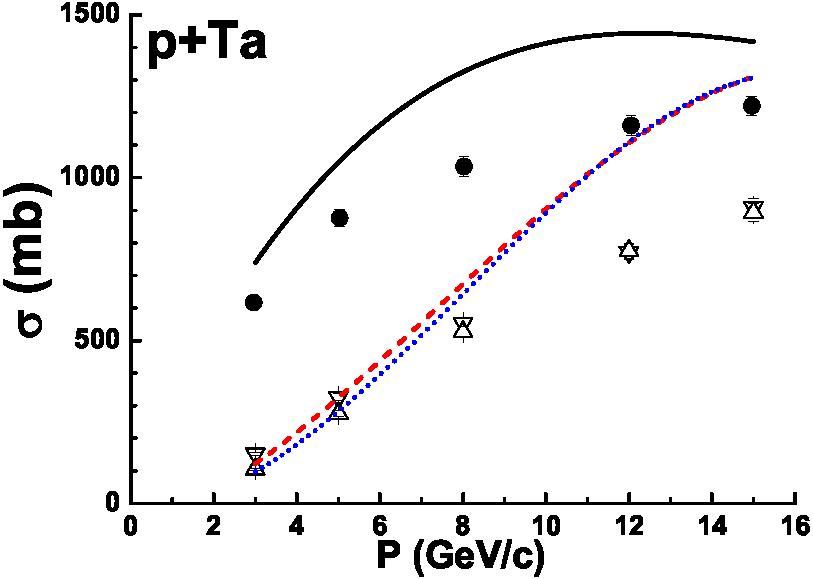
\includegraphics[height=1.8in,width=1.70in]{figures/FTFfig1_1.pdf}
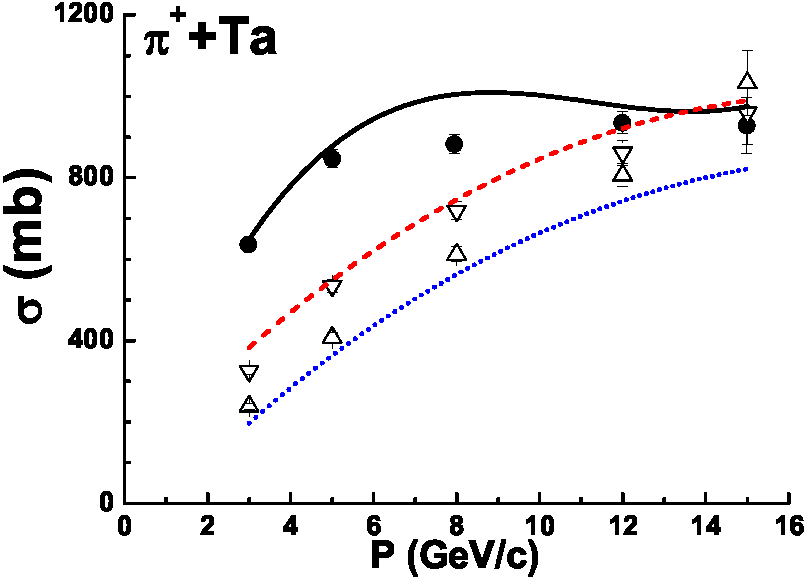
\includegraphics[height=1.8in,width=1.7in]{figures/FTFfig1_2.pdf}
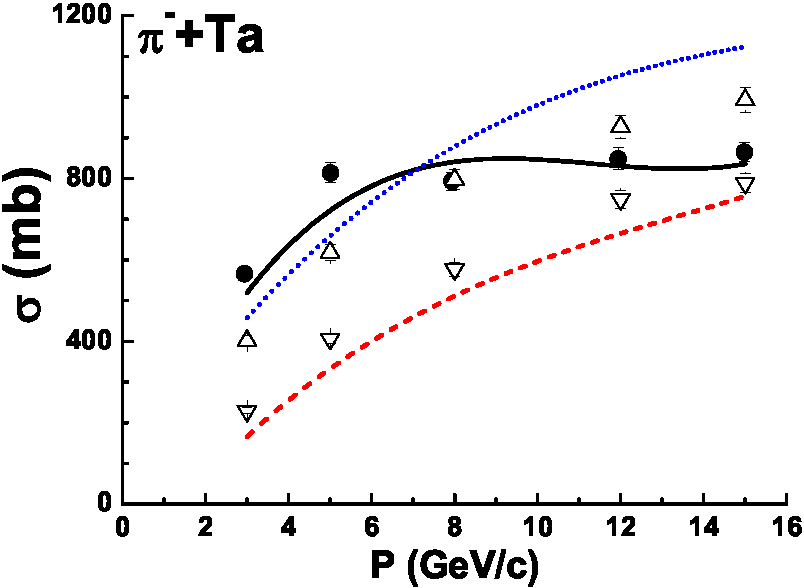
\includegraphics[height=1.8in,width=1.7in]{figures/FTFfig1_3.pdf}
\caption{Inclusive cross sections for $p$, $\pi^+$ and $\pi^-$ production in
         $p{\rm Ta}$, $\pi^+{\rm Ta}$ and $\pi^-{\rm Ta}$ interactions as a 
         function of projectile hadron momentum.  Data from the HARP-CDP 
         group \protect{\cite{hadbib:FTF17}} are shown as closed circles for
         protons and up- and down-triangles for $\pi^+$ and $\pi^-$,
         respectively.  Lines are FTF model calculations: solid for protons,
         dashed and short-dashed for $\pi^+$ and $\pi^-$, respectively.}
\label{had:FTFfig1}
\end{figure}


  \label{had:string}


%\subsubsection{Nuclear de-excitation model}
% \label{sec:evaporation}

% %%%%%%%%%%%%%%%%%%%%%%%%%%%%%%%%%%%%%%%%%%%%%%%%%%%
% precompound.tex
% Author: Jose-Manuel Quesada
%%%%%%%%%%%%%%%%%%%%%%%%%%%%%%%%%%%%%%%%%%%%%%%%%%%
\paragraph{The precompound model}
The native \Gfour{} pre-equilibrium  model is based on a version of the 
semi-classical exciton model \cite{hadbib:gudima83} and is used as the back-end
stage of several cascade and quark-gluon string generators.  It handles the 
de-excitation of the remnant nucleus from its formation immediately following a
cascade or high energy collision, until it reaches equilibrium.  During this 
time, internal transitions of the pre-compound nuclear system compete with 
nucleon and light cluster emissions.  The passage to the state of statistical 
equilibrium, which happens when the transition probabilities for increasing and 
decreasing the exciton number become approximately equal (equilibrium condition),
is roughly characterized by an equilibrium number of excitons $n_{eq}$.  In the
simulation $n_{eq}$ is a calculated number based on the assumption that the 
equilibrium condition is met. 

Some refinements were introduced recently 
\cite{hadbib:calor-2008, hadbib:ijrb-space-2012, hadbib:iaea-spa-2009}, 
namely more realistic inverse cross section parameterizations and combinatorial
factors for particle emission, a phenomenological parameterization of the 
transition matrix elements, and a more physically consistent condition for the 
transition to equilibrium, since in certain circumstances this condition is 
reached well before the previously used rough estimate of $n_{eq}$.

At the end of the pre-equilibrium stage, the residual nucleus should be left in
an equilibrium state, in which the excitation energy is shared by the entire 
nuclear system.  Such an equilibrated compound nucleus is characterized by its 
mass, charge and excitation energy with no further memory of the steps which led
to its formation.



% %%%%%%%%%%%%%%%%%%%%%%%%%%%%%%%%%%%%%%%%%%%%%%%%%%%%%%%%%%%%%%%%%%%
% deexcitation.tex
% Authors: Vladimir Ivantchenko, Jose Manuel Quesada, Gunter Folger
%%%%%%%%%%%%%%%%%%%%%%%%%%%%%%%%%%%%%%%%%%%%%%%%%%%%%%%%%%%%%%%%%%%
\paragraph{Nuclear de-excitation models}
The final de-excitation of a nucleus to a thermalized state is simulated by
several semi-classical models which are responsible for sampling the 
multiplicity of neutrons, protons, light ions, isotopes, and photons.  They
are:
\begin{itemize}
\item Fermi break-up (FBU) \cite{hadbib:mfm-bondorf-1995},
\item statistical multifragmentation \cite{hadbib:mfm-bondorf-1995},
\item fission, based on the Bohr-Wheeler semi-classical model 
      \cite{hadbib:jinr-fis-1977, hadbib:inr-fis-1993},
\item evaporation of nucleons and light fragments, which is handled by models 
      based on either
\begin{itemize}
  \item the Weisskopf-Ewing model \cite{hadbib:weisskopf-1940} for fragments up
        to and including $\alpha$ particles, or
  \item the generalized evaporation model (GEM) \cite{hadbib:gem-2001} for the 
        emission of fragments with masses up to $^{28}$Mg, and 
\end{itemize}
\item \gclass{G4PhotonEvaporation}, which simulates the emission of  
\begin{itemize}
\item discrete gammas according to the E1, M1 and E2 transition probabilities
      taken from the PhotonEvaporation database, which in turn is based on 
      the Evaluated Nuclear Structure Data File (ENSDF) \cite{hadbib:ENSDF}, 
      and 
\item continuous gammas according to the E1 giant dipole resonance strength 
      distribution.
\end{itemize}
\end{itemize}

These models are managed by the \gclass{G4ExcitationHandler} class, in which
they may be invoked in complement or sometimes concurrently with each other.
Some of them have been thoroughly validated and have undergone continuous 
improvement in recent years \cite{hadbib:calor-2008, hadbib:pmb-fluka-g4-2011}.

In order to properly describe the double differential cross sections and isotope
production data of the IAEA spallation benchmark 
\cite{hadbib-iaea-spa-benchmark,hadbib:iaea-spa-2009}, the standard and GEM 
models were combined to form a hybrid model, and the fission model was improved
\cite{hadbib:pnst-preco-2011,hadbib:ijrb-space-2012,hadbib:iaea-spa-2009}.

For radiobiological applications it is essential that the FBU model be used by 
default for the de-excitation of light fragments (Z $<$ 9, A $<$ 17), taking 
into account Pauli blocking and all possible decay channels into stable and 
long-lived fragments.  Validations
\cite{hadbib:nima-pshenich-2010,hadbib:pmb-fluka-g4-2011}
triggered many of the refinements to this model.

For proton and ion beam therapy applications, the photon evaporation model, 
which is critical for the tracking of the Bragg peak from emitted prompt gammas, 
was improved \cite{hadbib:prompt-gamma-2014}.  The statistical 
multifragmentation model, responsible for the explosive break-up of heavier hot
nuclei  (Z $>$ 8, A $>$ 16, and excitation energy $>$ 3 MeV/u), is relevant 
in simulations of shielding from cosmic radiation and has also been validated
\cite{hadbib:ijrb-space-2012,hadbib:nima-pshenich-2010}. 

 \label{had:deexcitation}

% needs discussion of G4NuclNuclDiffuseElastic
%%%%%%%%%%%%%%%%%%%%%%%%%%%%%%%%%%%%%%%%%%%%%%%%%%%%%
% nucleusnucleus.tex
% Authors: Davide Mancusi, Dennis Wright
%%%%%%%%%%%%%%%%%%%%%%%%%%%%%%%%%%%%%%%%%%%%%%%%%%%%%
\paragraph{Nucleus-nucleus models}
As of release 10.0 there were six \Gfour{} models capable of handling
nucleus-nucleus collisions: binary light ion, abrasion/ablation, 
electromagnetic dissociation, QMD, INCL++ and FTF models.

The Binary Light Ion model handles collisions in which either the projectile or
the target has mass $A < 13$.  Based on the \Gfour{} Binary Cascade model 
\cite{hadbib:binary}, it is valid above 80 MeV and below 10 GeV/nucleon. 

Operating over a similar energy range, but without limits on the projectile or
target masses, the \gclass{G4WilsonAbrasion} model, based on NUCFRG2 
\cite{hadbib:wilson} is faster, but less detailed, than the Binary Light Ion 
model.  It is a geometrical model in which a portion of the target nucleus along
the incident path of the projectile is gouged out, forming a forward-going 
compound nucleus and a residual target.  The associated Wilson ablation model is
used to de-excite the products of the initial collision.

Also based on NUCFRG2, \gclass{G4EMDissociation} is an electromagnetic 
dissociation model provided to handle the production of nuclear fragments 
resulting from the exchange of virtual photons between projectile and target 
nuclei.  This model is valid for nuclei of all masses and all energies.
  
QMD (Quantum Molecular Dynamics) is a native \Gfour{} model based on an extension
of the classical molecular dynamics model introduced in release 9.1.  Each 
nucleon in the target and projectile nuclei is treated as a gaussian wave packet
which propagates with scattering through the nuclear medium, taking Pauli 
exclusion into account.  The nuclear potential is that of two merging nuclei and
its shape is re-calculated at each time step of the collision.  
Participant-participant scattering is also taken into account.  
These last two facts combine to make the model rather slow for collisions of
heavy nuclei, but the production of nuclear fragments versus energy is well 
reproduced.  The model is valid for all projectile-target combinations and for
projectile energies between 100 MeV/nucleon and 10 GeV/nucleon.  Since its
introduction, the model was made Lorentz covariant and improvements were made in
fragment prodcution at relativistic energies.
 
The \inclxx\ model, covered above, can also accommodate nucleus-nucleus 
reactions provided the projectile has a mass below $A = 19$ and an energy 
between 1 MeV/nucleon and 3 GeV/nucleon.  A broad validation campaign on 
heterogeneous observables has shown that, in spite of the conceptual 
difficulties, the extended \inclxx\ model yields predictions in fair agreement 
with experimental data; it is however crucial to make a suitable choice for the 
coupling with the statistical de-excitation model.

The FTF model, covered above, is capable of modeling 
reactions with all combinations of projectile and target mass, with projectile 
energies in the range 2 GeV/nucleon to about 1 TeV/nucleon.  However, validation
of this application is still in progress, and collisions of two heavy nuclei are 
expected to be computationally expensive.



%%%%%%%%%%%%%%%%%%%%%%%%%%%%%%%%%%%%%%%%%%%%%%%%%%%
% radioactivedecay.tex
% Author: Dennis Wright
%%%%%%%%%%%%%%%%%%%%%%%%%%%%%%%%%%%%%%%%%%%%%%%%%%%
\paragraph{The radioactive decay process}
The \gclass{G4RadioactiveDecay} process and model handles $\alpha$, $\beta^-$,
$\beta^+$, isomeric transition (IT) and electron capture (EC) decays, and can be
applied to generic ions both in flight and at rest.   

Details for each decay or level transition, such as nuclear level energies, 
branching ratios and reaction Q values, come from the \Gfour{} RadioactiveDecay 
database, which currently contains entries for 2798 nuclides.  Details of 
specific gamma levels used for IT decays are taken from the \Gfour{} 
PhotonEvaporation database.  Both the PhotonEvaporation and RadioactiveDecay 
databases take their data from the Evaluated Nuclear Structure Data File (ENSDF)
\cite{hadbib:ENSDF} and have recently been rationalized so that their common 
nuclear levels have identical values.

Beginning with \Gfour{} release 9.6 and continuing through releases currently in
preparation, a number of improvments have been made to the radioactive decay 
package.  These include:

\begin{itemize}
\item a complete review of the PhotonEvaporation and RadioactiveDecay databases,
      and updating to the 2013 version of ENSDF,
\item the ability to model decays with lifetimes as short as 1 ps,
\item decays of observationally stable ground states, that is, those having
      very long predicted life times, but which have not yet been observed to 
      decay,  
\item the addition of unique first, second and third forbidden $\beta^-$ and
      $\beta^+$ decays,
\item the default invocation of the atomic relaxation model after IT and EC 
      decays, and 
\item improved energy conservation for all decay modes.
\end{itemize}



%%%%%%%%%%%%%%%%%%%%%%%%%%%%%%%%%%%%%%%%%%%%%%%%%%%
% gamleptnuclear.tex
% Authors: Dennis Wright, Mike Kelsey
%%%%%%%%%%%%%%%%%%%%%%%%%%%%%%%%%%%%%%%%%%%%%%%%%%%
\paragraph{Gamma- and lepto-nuclear models}
Due to the relatively small electromagnetic coupling, gamma- and lepto-nuclear
reactions play a small role in high energy physics calorimetry. They are 
important, though, for nuclear, medium energy and cosmic ray physics.  For this 
reason \Gfour{} models for these reactions were extended and improved.  

The \gclass{G4PhotoNuclearProcess} is implemented by two models, the Bertini 
cascade below 3.5 GeV and the Quark-Gluon-String (QGS) model above 3 GeV.  Both
models treat the incident gamma as if it were a hadron interacting with a 
nucleon within the nuclear medium.  Nevertheless, below 30 MeV the Bertini model
does capture some collective nuclear effects such as the giant dipole resonance.

Both the electro-nuclear and muon-nuclear models
(\gclass{G4ElectroVD\allowbreak{}Nuclear\allowbreak{}Model}
and \gclass{G4MuonVD\allowbreak{}Nuclear\allowbreak{}Model}) exploit two
features of the hybrid electromagnetic hadronic interaction: the factorization
of the interaction into separate hadronic and electromagnetic parts and the 
treatment of the exchanged 
photon as if it were a hadron.  The electromagnetic vertex produces a virtual 
photon from a two-dimensional cross section table and uses the method of 
equivalent photons to make the photon real.  As in the photo-nuclear case 
mentioned above, the photon is then treated as a hadron for the remainder of the
interaction.  For real photons below 10 GeV the Bertini cascade handles the 
interaction;  above 10 GeV the photon is converted to a neutral pion and the 
interaction proceeeds using the FTF string model.

 \label{had:gamleptnucleus}

%%%%%%%%%%%%%%%%%%%%%%%%%%%%%%%%%%%%%%%%%%%%%%%%%%%
% obsoletemodels.tex
% Author: Dennis Wright
%%%%%%%%%%%%%%%%%%%%%%%%%%%%%%%%%%%%%%%%%%%%%%%%%%%
\paragraph{Obsolete models}
The first \Gfour{} hadronic models, the Low Energy Parameterized (LEP) and 
High Energy Parameterized (HEP), were both re-engineered versions of the Fortran
code Gheisha \cite{hadbib:gheisha}.  In their original form they were designed
and tuned to reproduce high energy shower shapes.  They conserved energy on
average, but not on an event-by-event basis.  With the advent of more 
theoretically detailed models, both LEP and HEP models were removed from version
10.0 of the toolkit.

Prior to \Gfour{} 10.0, a number of models and cross section sets dealing
with nuclear de-excitation, hadron capture, gamma-nuclear and lepton-nuclear 
reactions were implemented by the Chiral Invariant Phase Space (CHIPS) package.
Since version 10.0, most of these reactions have been implemented by other models 
although some of the cross sections still maintain the original CHIPS coding.

Lastly, the isotope production model, used to count recoil nuclei produced in
various reactions, was removed in version 10.0, as all hadronic models now 
produce recoil nuclei explicitly.



